% !TeX root = ../../Book3.tex
% 纲要标题：## 第4章　子流形、法丛与相容方程
% 纲要位置：几何学计划纲要.md，第 2226 行。
% 正文状态：初稿；尚未正式审核。

% 纲要内容开始
% 
% > 本章目标与证明范围：把第一卷曲面的两个基本形式推广到高余维。完整证明 Gauss、Codazzi、Ricci 方程及所选空间形式中的局部实现；法联络不作为附带记号。
% 
% 纲要内容结束

\chapter{子流形、法丛与相容方程}
\label{g3:ch:04}
\BookChapterNumber{g3:ch:04}

\begin{chapterabstract}
	浸入的诱导度量描述切向长度，第二基本形式和法联络描述切空间与法空间在环境中的变化。本章建立任意余维的切法分解，完整推导 Gauss、Codazzi 和 Ricci 方程，并将空间形式中的三组相容条件组织成一个平坦联络。通过局部平行标架与位置一形式的积分，构造所给数据的等距浸入，证明其在环境等距意义下的唯一性，并辨明整体延拓中的环路返回与周期障碍。球面、乘积和管状模型用于计算主曲率与内在曲率，面积一阶变分则解释平均曲率向量的几何意义。
\end{chapterabstract}

\begin{learninggoals}
	\begin{itemize}
		\item 从环境导数的切向与法向投影构造第二基本形式、形算子和法联络，核对它们的对应关系与符号。
		\item 完整证明三组相容方程，说明高余维中法曲率方程所增加的独立条件。
		\item 从相容数据构造 Euclid、球面及双曲模型中的局部浸入，解释唯一性的完整数据条件及整体单值障碍。
		\item 计算主曲率、管状体积和面积的一阶变化，将极小性与平均曲率、位置向量的 Laplace 公式相联系。
	\end{itemize}
\end{learninggoals}

把一个平面条带卷成圆柱，可以保持条带内的长度和夹角，却改变它在三维空间中的形状。平面与圆柱的 Gauss 曲率同为零；沿圆柱绕轴方向移动时，切平面不断转动，而沿平面移动时没有这种变化。内在曲率已经说明度量自身如何偏离平直，但要恢复浸入，还需要记录环境方向中的变化。

\ProseParagraphBreak

曲面在三维空间中只有一条法线方向，形算子便足以把法向变化写成切向量。高余维时，法空间本身也可以在各法向方向之间转动。它的导数和曲率分别由法联络及法曲率记录；第二基本形式将切方向与法方向联系起来。把环境曲率按切、法两部分展开，会得到必须同时满足的 Gauss、Codazzi 与 Ricci 方程。\footnote{Delfino Codazzi（1824--1873），意大利数学家，研究曲面理论与曲线坐标。}反过来，这些方程是否足以产生一个实际浸入，是本章的主要存在问题。

\ProseParagraphBreak

本章使用前三章的 Levi-Civita 联络、曲率张量、指数映射及散度定理，并回顾向量丛局部标架所需的记号。局部实现使用光滑线性常微分方程的初值唯一性与参数依赖；相关结论在第一卷第13.1节已证明，本章给出将它们用于多变量相容系统的步骤。第一卷曲面理论中的两个基本形式将在任意余维重新建立。各几何对象均光滑；边界、紧性、单连通性以及法向的整体可选性按具体结果说明。

\ProseParagraphBreak

本章固定 \(B(X,Y)=(\bar\nabla_X\mathrm df(Y))^\perp\)、\(g(A_\xi X,Y)=\langle B(X,Y),\xi\rangle\)，并取平均曲率向量 \(H=n^{-1}\operatorname{tr}_g B\)。因此球面的外法向形算子为负，而球面的内在截面曲率为正。曲率方向及四阶张量次序沿用第三章。球面与球面乘积的内在度量模型可对照 Petersen 第3版第4.2.1--4.2.2节\cite[第4.2.1--4.2.2节]{Petersen2016}；本章进一步计算它们在不同环境中的法向数据。

% !TeX root = ../../Book3.tex
% 纲要标题：### 4.1 切向与法向分解
% 纲要位置：几何学计划纲要.md，第 2230 行。
% 正文状态：初稿；尚未正式审核。

% 纲要内容开始
% 
% * 第二基本形式和形算子
% * 法联络及其曲率
% * 平均曲率向量
% * 全测地和全脐子流形
% 
% 纲要内容结束

\section{切向与法向分解}
\label{g3:sec:0401}

沿子流形移动一个切向量，环境中的导数可能离开切空间。第一章将导数的切向部分识别为诱导度量的 Levi-Civita 联络，现在保留下来的法向部分记录浸入怎样弯曲。法向量自身也会变化：它的切向导数由同一弯曲数据决定，法向导数则构成法丛上的联络。余维大于一时，法向空间中还有独立的转动，必须把这部分一起记录。

\subsection{第二基本形式和形算子}
\label{g3:subsec:0401:01}

设 \(f:(M^n,g)\to(\bar M^{n+r},\bar g)\) 为光滑等距浸入，其中 \(n\ge1\)，两流形均无边界，且 \(g=f^*\bar g\)。沿 \(f\) 的向量场，是给每个源点 \(p\) 指定一个向量 \(W(p)\in\mathrm{T}_{f(p)}\bar M\) 的光滑截面。它们所在的丛记为 \(f^*\mathrm{T}\bar M\)。即使两个不同源点有同一个像，这两个源点上的纤维仍分别记录。

\begin{definition}\label{g3:def:normal-bundle}
	设 \(f:(M^n,g)\to(\bar M^{n+r},\bar g)\) 为光滑等距浸入。其\term[facong]{法丛}[normal bundle]为
	\[
		N_fM\coloneqq
		\{(p,\xi):p\in M,\ \xi\in\mathrm{T}_{f(p)}\bar M,\
			\bar g(\xi,\mathrm df_p(v))=0
			\text{ 对所有 }v\in\mathrm{T}_pM\}.
	\]
	其截面称为法向量场。正交分解记为
	\[
		f^*\mathrm{T}\bar M=\mathrm df(\mathrm{T}M)\oplus N_fM,
		\qquad W=W^\top+W^\perp.
	\]
\end{definition}
\symidx{\(N_fM\)}

这个分解随点光滑。事实上，在源坐标中令 \(f_i=\mathrm df(\partial_i)\)，则切向投影为
\[
	W^\top=\sum_{i,j}g^{ij}\bar g(W,f_i)f_j.
\]
矩阵 \((g^{ij})\) 光滑，故两个投影均光滑，法向投影具有常秩 \(r\)。局部选择线性无关的投影像，再作光滑正交化，就得到法丛的局部正交单位标架。

\ProseParagraphBreak

沿 \(f\) 的环境协变导数采用\cref{g3:prop:induced-connection-projection}中的定义。若 \(f^a=y^a\circ f\)、\(W=W^a\partial_{y^a}|_f\)，则
\[
	\bar\nabla^f_XW
	=\left(X(W^a)+\bar\Gamma^a_{bc}(f)\,X(f^b)W^c\right)
		\partial_{y^a}|_f.
\]
它只使用沿 \(f\) 的数据。以下将 \(\bar\nabla^f_X\) 简写为 \(\bar\nabla_X\)，其中 \(X\) 始终是源流形上的向量场。这一联络满足环境度量的乘积规则，而上述命题给出
\[
	(\bar\nabla_X\mathrm df(Y))^\top=\mathrm df(\nabla_XY).
\]

\begin{definition}\label{g3:def:second-fundamental-form}
	设 \(f:(M^n,g)\to(\bar M,\bar g)\) 为光滑等距浸入。定义它的\term[dierjibenxingshi]{第二基本形式}[second fundamental form]为法丛值的二阶协变张量
	\[
		B(X,Y)\coloneqq(\bar\nabla_X\mathrm df(Y))^\perp.
	\]
\end{definition}
\symidx{\(B\)}

\begin{proposition}\label{g3:prop:gauss-decomposition}
	光滑等距浸入 \(f:(M,g)\to(\bar M,\bar g)\) 的第二基本形式光滑、对称，并对两个输入都为 \(C^\infty(M)\) 线性。切向与法向分解给出
	\begin{equation}\label{g3:eq:gauss-decomposition}
		\bar\nabla_X\mathrm df(Y)=\mathrm df(\nabla_XY)+B(X,Y).
	\end{equation}
\end{proposition}
\begin{proof}
	对光滑函数 \(h\)，第一输入的函数线性直接来自联络；第二输入则满足
	\[
		\bar\nabla_X\mathrm df(hY)
		=X(h)\mathrm df(Y)+h\bar\nabla_X\mathrm df(Y).
	\]
	第一项切向，取法向投影后为零，故 \(B(X,hY)=hB(X,Y)\)。各投影和联络系数光滑，因而 \(B\) 光滑。

	环境联络的无挠性沿浸入表现为
	\[
		\bar\nabla_X\mathrm df(Y)-\bar\nabla_Y\mathrm df(X)
		=\mathrm df([X,Y]).
	\]
	可由上面的坐标公式直接核对：含 \(\bar\Gamma^a_{bc}\) 的两项因下指标对称而相消，余下分量为 \(X(Yf^a)-Y(Xf^a)=[X,Y]f^a\)。右侧切向，取法向投影即得 \(B(X,Y)=B(Y,X)\)。最后将环境导数分成两个正交分量，切向部分由诱导联络公式给出，得到式\eqref{g3:eq:gauss-decomposition}。
\end{proof}

式\eqref{g3:eq:gauss-decomposition}称为 Gauss 公式。它把内在联络与浸入的额外二阶数据分开。反过来，对法向场求导，也会出现切向分量；由于切向场与法向场的内积恒为零，这个分量已由 \(B\) 决定。

\begin{definition}\label{g3:def:shape-operator}
	设 \(f:(M,g)\to(\bar M,\bar g)\) 为光滑等距浸入。对法向量 \(\xi\in N_{f,p}M\)，定义\term[xingsuanzi]{形算子}[shape operator]
	\(A_\xi:\mathrm{T}_pM\to\mathrm{T}_pM\)，使
	\begin{equation}\label{g3:eq:shape-operator-pairing}
		g(A_\xi X,Y)=\bar g(B(X,Y),\xi)
		\qquad(X,Y\in\mathrm{T}_pM).
	\end{equation}
	正定内积保证这个线性算子存在且唯一。
\end{definition}
\symidx{\(A_\xi\)}

\begin{proposition}\label{g3:prop:weingarten-decomposition}
	设 \(f:(M,g)\to(\bar M,\bar g)\) 为光滑等距浸入。形算子随 \(\xi\) 线性变化，且每个 \(A_\xi\) 都自伴。对光滑法向场 \(\xi\)，令
	\(\nabla^\perp_X\xi=(\bar\nabla_X\xi)^\perp\)，则
	\begin{equation}\label{g3:eq:weingarten-formula}
		\bar\nabla_X\xi=-\mathrm df(A_\xi X)+\nabla^\perp_X\xi.
	\end{equation}
\end{proposition}
\begin{proof}
	关于 \(\xi\) 的线性由式\eqref{g3:eq:shape-operator-pairing}及唯一性得到。在坐标中，\((A_\xi)^i{}_j=g^{ik}\bar g(B(\partial_j,\partial_k),\xi)\)，故对光滑法向场，形算子场也光滑。由 \(B\) 对称，
	\[
		g(A_\xi X,Y)=\bar g(B(X,Y),\xi)
		=\bar g(B(Y,X),\xi)=g(X,A_\xi Y),
	\]
	所以 \(A_\xi\) 自伴。对恒等式 \(\bar g(\xi,\mathrm df(Y))=0\) 沿 \(X\) 求导，得到
	\[
		\bar g(\bar\nabla_X\xi,\mathrm df(Y))
		=-\bar g(\xi,\bar\nabla_X\mathrm df(Y))
		=-g(A_\xi X,Y).
	\]
	这对所有 \(Y\) 成立，故切向分量是 \(-\mathrm df(A_\xi X)\)；余下分量正是所定义的 \(\nabla^\perp_X\xi\)。
\end{proof}

式\eqref{g3:eq:weingarten-formula}称为\term[weingartengongshi]{Weingarten 公式}[Weingarten formula]。\footnote{Julius Weingarten（1836--1910），德国数学家，研究曲面等距变形与曲率线。}其负号来自正交关系的求导。若余维为一，取局部单位法向 \(\nu\)，则 \(\bar\nabla_X\nu\) 与 \(\nu\) 正交，已没有法向分量，所以 \(\bar\nabla_X\nu=-\mathrm df(A_\nu X)\)。

\begin{example}\label{g3:exm:sphere-extrinsic-sign}
	对半径 \(a>0\) 的圆球面 \(S^n(a)\subset\mathbb R^{n+1}\)，取外向单位法向 \(\nu(p)=p/a\)。环境联络为普通导数，故对切向量 \(X\)，
	\[
		\mathrm D_X\nu=\frac1aX,\qquad
		A_\nu=-\frac1a\operatorname{id},\qquad
		B(X,Y)=-\frac1a g(X,Y)\nu.
	\]
	这些等式直接来自法向的变化，与第一章球面诱导联络的符号相容。把 \(\nu\) 改为 \(-\nu\) 会改变 \(A_\nu\) 的符号，但不改变法丛值张量 \(B\)。
\end{example}

\subsection{法联络及其曲率}
\label{g3:subsec:0401:02}

法向导数中的切向部分已经由 \(B\) 决定，余下部分比较的是相邻法向空间中的向量。余维为一时，单位法向的这部分导数为零；余维较高时，保持长度的法向量还可以在法向空间内部转动。

\begin{definition}\label{g3:def:normal-connection}
	设 \(f:(M,g)\to(\bar M,\bar g)\) 为光滑等距浸入。法丛上的\term[falianluo]{法联络}[normal connection]定义为
	\[
		\nabla^\perp_X\xi=(\bar\nabla_X\xi)^\perp,
		\qquad \xi\in\Gamma(N_fM).
	\]
	法向场 \(\xi\) 若满足 \(\nabla^\perp_X\xi=0\) 对所有 \(X\) 成立，则称为法平行的。
\end{definition}
\symidx{\(\nabla^\perp\)}

\begin{proposition}\label{g3:prop:normal-connection-metric}
	光滑等距浸入的 \(\nabla^\perp\) 是法丛上的光滑联络，并与法丛上的诱导内积相容，即
	\begin{equation}\label{g3:eq:normal-connection-metric}
		X\bar g(\xi,\zeta)
		=\bar g(\nabla^\perp_X\xi,\zeta)
			+\bar g(\xi,\nabla^\perp_X\zeta).
	\end{equation}
\end{proposition}
\begin{proof}
	正交投影为光滑丛映射，环境联络对求导方向为函数线性，所以
	\[
		\nabla^\perp_{hX}\xi=h\nabla^\perp_X\xi,\qquad
		\nabla^\perp_X(h\xi)=X(h)\xi+h\nabla^\perp_X\xi.
	\]
	与实线性一起，这正是丛联络的各项公理。环境度量相容性给出
	\[
		X\bar g(\xi,\zeta)
		=\bar g(\bar\nabla_X\xi,\zeta)+\bar g(\xi,\bar\nabla_X\zeta).
	\]
	这里 \(\xi,\zeta\) 都法向，另一个输入的切向分量不贡献内积，因此可将两个环境导数都替换为其法向投影，得到式\eqref{g3:eq:normal-connection-metric}。
\end{proof}

\begin{definition}\label{g3:def:normal-curvature}
	光滑等距浸入的\term[faqulv]{法曲率}[normal curvature]为法丛联络的曲率
	\begin{equation}\label{g3:eq:normal-curvature-definition}
		R^\perp(X,Y)\xi
		\coloneqq\nabla^\perp_X\nabla^\perp_Y\xi
			-\nabla^\perp_Y\nabla^\perp_X\xi
			-\nabla^\perp_{[X,Y]}\xi.
	\end{equation}
	若 \(R^\perp=0\)，称法联络平坦。
\end{definition}
\symidx{\(R^\perp\)}

\begin{proposition}\label{g3:prop:normal-connection-curvature}
	设 \(f:(M,g)\to(\bar M,\bar g)\) 为光滑等距浸入。\(R^\perp(X,Y)\xi\) 对 \(X,Y,\xi\) 均为函数线性，对 \(X,Y\) 反对称，且在法向输入上满足
	\begin{equation}\label{g3:eq:normal-curvature-skew}
		\bar g(R^\perp(X,Y)\xi,\zeta)
		=-\bar g(\xi,R^\perp(X,Y)\zeta).
	\end{equation}
	因而 \(R^\perp\) 是取值于法丛斜自伴算子的二形式。
\end{proposition}
\begin{proof}
	反对称性来自定义。对光滑函数 \(h\)，利用
	\([hX,Y]=h[X,Y]-Y(h)X\)，展开第一输入得
	\[
		\begin{aligned}
			R^\perp(hX,Y)\xi
			={}&h\nabla^\perp_X\nabla^\perp_Y\xi
				-\nabla^\perp_Y(h\nabla^\perp_X\xi)\\
			&-h\nabla^\perp_{[X,Y]}\xi
				+Y(h)\nabla^\perp_X\xi
			=hR^\perp(X,Y)\xi.
		\end{aligned}
	\]
	第二输入的函数线性由反对称性得到。对于法向输入，
	\[
		\nabla^\perp_X\nabla^\perp_Y(h\xi)
		=X(Yh)\xi+(Yh)\nabla^\perp_X\xi
			+(Xh)\nabla^\perp_Y\xi
			+h\nabla^\perp_X\nabla^\perp_Y\xi.
	\]
	交换 \(X,Y\) 并减去括号方向的导数后，函数的二阶导数合成为
	\(XYh-YXh-[X,Y]h=0\)，两个交叉项也抵消，因此第三输入函数线性。局部标架展开说明它只取决于各输入在一点的值，并且光滑。

	最后将度量相容式连续使用两次：
	\[
		\begin{aligned}
			XY\bar g(\xi,\zeta)
			={}&\bar g(\nabla^\perp_X\nabla^\perp_Y\xi,\zeta)
				+\bar g(\nabla^\perp_Y\xi,\nabla^\perp_X\zeta)\\
			&+\bar g(\nabla^\perp_X\xi,\nabla^\perp_Y\zeta)
				+\bar g(\xi,\nabla^\perp_X\nabla^\perp_Y\zeta).
		\end{aligned}
	\]
	交换 \(X,Y\) 后中间两项相消，再减去 \([X,Y]\bar g(\xi,\zeta)\)，左侧为零，右侧为式\eqref{g3:eq:normal-curvature-skew}两边移到一起的和。
\end{proof}

在局部正交单位法标架 \(\nu=(\nu_1,\ldots,\nu_r)\) 中，定义一形式矩阵 \(\eta=(\eta^\alpha{}_\beta)\)，使
\begin{equation}\label{g3:eq:normal-connection-matrix}
	\nabla^\perp\nu_\beta=\sum_\alpha\nu_\alpha\eta^\alpha{}_\beta,
	\qquad \eta^\alpha{}_\beta(X)=\bar g(\nabla^\perp_X\nu_\beta,\nu_\alpha).
\end{equation}
度量相容性给出 \(\eta^{\mathsf T}=-\eta\)。若法向场的列分量为 \(u\)，即 \(\xi=\nu u\)，则
\[
	\nabla^\perp_X\xi=\nu\bigl(Xu+\eta(X)u\bigr).
\]
因此平行性是关于各方向导数的方程 \(Xu=-\eta(X)u\)。

\begin{proposition}\label{g3:prop:normal-curvature-matrix}
	光滑等距浸入在局部正交单位法标架中的法曲率矩阵为
	\begin{equation}\label{g3:eq:normal-curvature-matrix}
		F^\perp=\mathrm d\eta+\eta\wedge\eta,\qquad
		R^\perp(X,Y)\nu_\beta
			=\sum_\alpha\nu_\alpha(F^\perp)^\alpha{}_\beta(X,Y).
	\end{equation}
	这里 \((\eta\wedge\eta)^\alpha{}_\beta
	=\sum_\gamma\eta^\alpha{}_\gamma\wedge\eta^\gamma{}_\beta\)。
\end{proposition}
\begin{proof}
	将式\eqref{g3:eq:normal-connection-matrix}代入曲率定义，\(\nu_\alpha\) 的系数为
	\[
		\begin{aligned}
			&X(\eta^\alpha{}_\beta(Y))
				-Y(\eta^\alpha{}_\beta(X))
				-\eta^\alpha{}_\beta([X,Y])\\
			&\qquad+\sum_\gamma
				\bigl(\eta^\alpha{}_\gamma(X)\eta^\gamma{}_\beta(Y)
				-\eta^\alpha{}_\gamma(Y)\eta^\gamma{}_\beta(X)\bigr).
		\end{aligned}
	\]
	第一行是 \(\mathrm d\eta^\alpha{}_\beta(X,Y)\)，第二行是矩阵外积的对应分量，故得到所述公式。
\end{proof}

局部正交单位法标架只要求每点的内积矩阵为单位矩阵。若进一步要求它在一个开邻域内法平行，就要求 \(\eta\) 在整个邻域为零，由式\eqref{g3:eq:normal-curvature-matrix}必有 \(R^\perp=0\)。下面的直接计算说明，这一要求对一般浸入不成立。

\begin{example}\label{g3:exm:nonflat-normal-connection}
	在 \(\mathbb R^4\) 中考虑图像浸入
	\[
		f(x,y)=\left(x,y,\frac{x^2}{2},xy\right).
	\]
	其坐标切向量为 \(f_x=(1,0,x,y)\)、\(f_y=(0,1,0,x)\)，以下两个场处处法向且线性无关：
	\[
		\xi_1=(-x,0,1,0),\qquad
		\xi_2=(-y,-x,0,1).
	\]
	它们不要求在整个邻域正交，在原点则为正交单位基。法向 Gram 矩阵及其行列式为
	\[
		G_N=
		\begin{pmatrix}1+x^2&xy\\xy&1+x^2+y^2\end{pmatrix},
		\qquad
		d_N=(1+x^2)(1+x^2+y^2)-x^2y^2>0.
	\]
	由于 \(\partial_y\xi_1=0\)，有 \(\nabla^\perp_{\partial_y}\xi_1=0\)。写
	\(\nabla^\perp_{\partial_x}\xi_1=a\xi_1+b\xi_2\)，对两法向场取内积便得
	\[
		G_N\binom{a}{b}=\binom{x}{y},\qquad
		a=\frac{x(1+x^2)}{d_N},\quad b=\frac{y}{d_N}.
	\]
	在原点 \(a=b=0\)、\(\partial_ya=0\)、\(\partial_yb=1\)，所以
	\[
		R^\perp(\partial_x,\partial_y)\xi_1\big|_{(0,0)}
		=-\nabla^\perp_{\partial_y}(a\xi_1+b\xi_2)\big|_{(0,0)}
		=-\xi_2(0,0)\ne0.
	\]
	因此任何包含原点的邻域都不存在处处法平行的法标架。环境空间本身平坦，并不使这个法联络平坦。
\end{example}

若法丛秩为一，任一局部单位法向 \(\nu\) 满足
\(\bar g(\nabla^\perp_X\nu,\nu)=0\)，而法向空间由 \(\nu\) 张成，故 \(\nabla^\perp\nu=0\)、\(R^\perp=0\)。这个局部结论不需要一个全局单位法向；是否能在整个流形选取这样的法向，是法线丛的另一项整体性质。

\subsection{平均曲率向量}
\label{g3:subsec:0401:03}

第二基本形式为每个切向方向给出一个法向弯曲向量。对正交方向求平均，应当得到不依赖所选切向基的法向量；这正是对 \(B\) 作度量迹的作用。

\begin{definition}\label{g3:def:mean-curvature-vector}
	设 \(f:(M^n,g)\to(\bar M,\bar g)\) 为光滑等距浸入，\(n\ge1\)。其\term[pingjunqulvxiangliang]{平均曲率向量}[mean curvature vector]为
	\begin{equation}\label{g3:eq:mean-curvature-vector}
		H\coloneqq\frac1n\operatorname{tr}_gB
			=\frac1n\sum_{i=1}^nB(e_i,e_i),
	\end{equation}
	其中 \(e_1,\ldots,e_n\) 为任意正交单位基。若 \(H\) 恒为零，称 \(f\) 为\term[jixiaojinru]{极小浸入}[minimal immersion]，相应浸入子流形称为极小子流形。
\end{definition}
\symidx{\(H\)}

若 \(e'_i=\sum_j e_jQ_{ji}\)，其中 \(Q\) 为正交矩阵，则
\[
	\sum_iB(e'_i,e'_i)
	=\sum_{j,k}\left(\sum_iQ_{ji}Q_{ki}\right)B(e_j,e_k)
	=\sum_jB(e_j,e_j).
\]
这既证明定义与正交基无关，也说明 \(H\) 是光滑法向场。在一般坐标中，
\[
	H=\frac1n g^{ij}B(\partial_i,\partial_j).
\]
与任意法向量 \(\xi\) 配对，式\eqref{g3:eq:shape-operator-pairing}又给出
\begin{equation}\label{g3:eq:mean-curvature-shape-trace}
	\bar g(H,\xi)=\frac1n\operatorname{tr}A_\xi.
\end{equation}
因此 \(H=0\) 等价于每个法向形算子都无迹。

\ProseParagraphBreak

对超曲面，选择单位法向 \(\nu\) 后可写 \(H=h\nu\)，其中 \(h=\operatorname{tr}A_\nu/n\) 是带符号的平均曲率。换成 \(-\nu\) 后，\(A_\nu\) 与 \(h\) 同时变号，向量 \(H\) 不变。由\cref{g3:exm:sphere-extrinsic-sign}，外向法向的圆球面满足
\[
	h=-\frac1a,\qquad H=-\frac1a\nu.
\]
平均曲率向量指向球心；它在这里采用平均值归一化，而非未除以维数的迹。

\begin{example}\label{g3:exm:curve-mean-curvature-vector}
	设 \(\gamma:I\to\bar M\) 为单位速光滑曲线，并给 \(I\) 度量 \(\mathrm ds^2\)。记 \(T=\dot\gamma\)。一维域中的单位坐标向量满足 \(\nabla_{\partial_s}\partial_s=0\)，所以 Gauss 公式给出
	\[
		B(\partial_s,\partial_s)=\bar{\mathrm D}_sT,\qquad
		H=\bar{\mathrm D}_sT.
	\]
	单位速条件使右侧与 \(T\) 正交。于是曲线的平均曲率向量就是其曲率向量，而单位速曲线是极小浸入当且仅当它是环境测地线。
\end{example}

\subsection{全测地和全脐子流形}
\label{g3:subsec:0401:04}

两种特殊弯曲情形可以直接用 \(B\) 描述。一种是所有方向都没有法向弯曲；另一种是所有单位切向方向的法向弯曲完全相同。前者对应测地线的保持，后者对应每个法向形算子都是数量算子。

\begin{definition}\label{g3:def:totally-geodesic-umbilical}
	设 \(f:(M^n,g)\to(\bar M,\bar g)\) 为光滑等距浸入，\(n\ge1\)。若 \(B\equiv0\)，称 \(f\) 为\term[quancedijinru]{全测地浸入}[totally geodesic immersion]。若每点 \(p\) 存在法向量 \(\zeta_p\)，使
	\[
		B_p(v,v)=g_p(v,v)\zeta_p\qquad
		\text{对所有 }v\in\mathrm{T}_pM,
	\]
	则称 \(f\) 为\term[quanqijinru]{全脐浸入}[totally umbilical immersion]。
\end{definition}

\begin{proposition}\label{g3:prop:totally-geodesic-characterization}
	设 \(f:(M,g)\to(\bar M,\bar g)\) 为光滑等距浸入。则 \(f\) 全测地，当且仅当每条 \(M\) 中的测地线经 \(f\) 映射后仍是保持原参数的环境测地线。此时，对每个 \(p\) 及足够小的 \(v\in\mathrm{T}_pM\)，有
	\begin{equation}\label{g3:eq:totally-geodesic-exponential}
		f(\exp_p^M v)=\exp_{f(p)}^{\bar M}(\mathrm df_pv).
	\end{equation}
\end{proposition}
\begin{proof}
	对任意光滑曲线 \(\gamma\)，将 Gauss 公式沿曲线使用，得到加速度分解
	\begin{equation}\label{g3:eq:immersion-curve-acceleration}
		\bar{\mathrm D}_t(\mathrm df(\dot\gamma))
		=\mathrm df(\mathrm D_t\dot\gamma)+B(\dot\gamma,\dot\gamma).
	\end{equation}
	具体地，在坐标中写 \(\dot\gamma=\dot x^i\partial_i\)，左侧为
	\(\ddot x^i f_i+\dot x^i\dot x^j\bar\nabla_{\partial_i}f_j\)；
	代入式\eqref{g3:eq:gauss-decomposition}，切向部分合成为
	\(\mathrm df((\ddot x^k+\Gamma^k_{ij}\dot x^i\dot x^j)\partial_k)\)，
	法向部分即上式所列的 \(B\)。

	若 \(B=0\)，当 \(\gamma\) 为测地线时，两项都为零，故 \(f\circ\gamma\) 是环境测地线。反过来，固定 \(p\) 及任意 \(v\in\mathrm{T}_pM\)。由\cref{g3:thm:geodesic-ivp}，存在以 \((p,v)\) 为初值的局部测地线。若其像也是环境测地线，在时间零代入加速度分解，得到 \(B_p(v,v)=0\)。由 \(B\) 对称，
	\[
		2B_p(v,w)=B_p(v+w,v+w)-B_p(v,v)-B_p(w,w)=0.
	\]
	所以 \(B=0\)。

	最后，在全测地情形，\(f\circ\gamma_{p,v}\) 与环境中以
	\((f(p),\mathrm df_pv)\) 为初值的测地线相同，这由同一初值唯一性得到。当 \(v\) 足够小，使两条曲线均定义到时间一时，比较时间一的值即得式\eqref{g3:eq:totally-geodesic-exponential}。
\end{proof}

\begin{proposition}\label{g3:prop:umbilical-characterization}
	设 \(f:(M^n,g)\to(\bar M,\bar g)\) 为光滑等距浸入，\(n\ge1\)。它全脐，当且仅当
	\begin{equation}\label{g3:eq:umbilical-second-fundamental-form}
		B(X,Y)=g(X,Y)H.
	\end{equation}
	这又等价于对每个法向量 \(\xi\)，有
	\[
		A_\xi=\bar g(H,\xi)\operatorname{id}.
	\]
	全脐浸入是全测地的，当且仅当其平均曲率向量为零。
\end{proposition}
\begin{proof}
	若 \(B_p(v,v)=g_p(v,v)\zeta_p\)，对 \(v+w\) 作同样计算，再减去 \(v,w\) 两式，得到
	\(B_p(v,w)=g_p(v,w)\zeta_p\)。在正交单位基中取迹，便有
	\(nH_p=n\zeta_p\)，所以 \(\zeta_p=H_p\)，得到式\eqref{g3:eq:umbilical-second-fundamental-form}。反向蕴含由令 \(Y=X\) 得到。

	将该式与任意 \(\xi\) 配对，形算子的定义给出
	\[
		g(A_\xi X,Y)=g(X,Y)\bar g(H,\xi),
	\]
	由度量非退化性得到数量算子表达。反过来，若所有 \(A_\xi\) 都具有这一形式，则 \(B(X,Y)-g(X,Y)H\) 与每个法向量正交；它本身法向，故为零。最后在全脐公式中令 \(H=0\) 即得 \(B=0\)，而 \(B=0\) 总使其迹 \(H\) 为零。
\end{proof}

Euclid 空间中的仿射子空间有常值切空间，环境导数的法向分量恒为零，因此全测地。圆球面由\cref{g3:exm:sphere-extrinsic-sign}满足 \(B=gH\)，故全脐，但它的 \(H\ne0\)，所以并非全测地。维数一时，每个单位切向量只差一个符号，任何曲线浸入都自动全脐；此时全测地与极小的条件则都要求曲率向量为零。
% 纲要条目排为编号小节标题，并进入目录与书签；说明段仍保留于纲要注释中。

% !TeX root = ../../Book3.tex
% 纲要标题：### 4.2 三组相容方程
% 纲要位置：几何学计划纲要.md，第 2134 行。
% 正文状态：未撰写；本文件目前是框架。

% 纲要内容开始
% 
% * Gauss 方程
% * Codazzi 方程
% * Ricci 法曲率方程
% * 高余维中不能删除的独立条件
% 
% 纲要内容结束

\section{三组相容方程}
\label{g3:sec:0402}

待撰写

\subsection{Gauss 方程}
\label{g3:subsec:0402:01}
待撰写

\subsection{Codazzi 方程}
\label{g3:subsec:0402:02}
待撰写

\subsection{Ricci 法曲率方程}
\label{g3:subsec:0402:03}
待撰写

\subsection{高余维中不能删除的独立条件}
\label{g3:subsec:0402:04}
待撰写
% 纲要条目排为编号小节标题，并进入目录与书签；说明段仍保留于纲要注释中。

% !TeX root = ../../Book3.tex
% 纲要标题：### 4.3 局部实现的结构方法
% 纲要位置：几何学计划纲要.md，第 2244 行。
% 正文状态：初稿；尚未正式审核。

% 纲要内容开始
% 
% * 给定度量、法丛及对称型
% * 标架系统及相容性
% * 空间形式中的局部基本定理
% * 唯一性及整体单值障碍
% 
% 纲要内容结束

\section{局部实现的结构方法}
\label{g3:sec:0403}

前三组方程是浸入所必须满足的条件，现在把问题反过来：若只给出长度、法方向及第二基本形式，能否把这些数据放进一个实际的环境空间？困难不在某一个点，而在相邻点的标架怎样同时移动。沿一条曲线可以解常微分方程；沿两个方向先后移动时，结果相容的条件正是 Gauss、Codazzi 与 Ricci 方程。下面将它们合成一个平坦联络，再由平行标架恢复位置。

\subsection{给定度量、法丛及对称型}
\label{g3:subsec:0403:01}

设 \(M^n\) 为无边界光滑流形，\(n\geq1\)。尚未有浸入时，“法丛”先只是一个抽象的实秩 \(r\geq0\) 光滑向量丛 \(E\to M\)，带正定纤维内积 \(\langle\ ,\ \rangle_E\) 和保持该内积的联络 \(\nabla^E\)。其余数据是光滑黎曼度量 \(g\) 和光滑对称双线性型
\[
	B\in\Gamma(\operatorname{Sym}^2\mathrm T^*M\otimes E).
\]
这时 \(B(X,Y)\) 已经指定“向哪个法方向弯曲”，但尚未把该法方向识别为某个环境切空间中的向量。记 \(\nabla\) 为 \(g\) 的 Levi-Civita 联络，按
\[
	g(A_\xi X,Y)=\langle B(X,Y),\xi\rangle_E
\]
定义自伴算子 \(A_\xi\)。秩 \(r=0\) 时，\(E,B,A\) 的各项均按零理解。

\ProseParagraphBreak

固定一个实数 \(c\)，表示待实现的环境截面曲率。上一节的空间形式相容方程在这些抽象数据上仍有意义：
\begin{align}
	\mathrm{Rm}(X,Y,Z,W)
	&=c\bigl(g(X,Z)g(Y,W)-g(X,W)g(Y,Z)\bigr)\notag\\
	&\quad+\langle B(X,Z),B(Y,W)\rangle_E
	-\langle B(X,W),B(Y,Z)\rangle_E,\label{g3:eq:abstract-gauss-data}\\
	(\nabla B)(X;Y,Z)&=(\nabla B)(Y;X,Z),\label{g3:eq:abstract-codazzi-data}\\
	\langle R^E(X,Y)\xi,\eta\rangle_E
	&=g([A_\xi,A_\eta]X,Y).\label{g3:eq:abstract-ricci-data}
\end{align}
这里
\[
	(\nabla B)(X;Y,Z)
	=\nabla^E_X(B(Y,Z))-B(\nabla_XY,Z)-B(Y,\nabla_XZ),
\]
而 \(R^E(X,Y)=\nabla^E_X\nabla^E_Y-\nabla^E_Y\nabla^E_X-\nabla^E_{[X,Y]}\)。三式分别对应\cref{g3:cor:space-form-compatibility}中的切向、混合与法向相容条件。

\ProseParagraphBreak

为明确实现的目标，令 \(N=n+r\)，并记 \(Q_c^N\) 为以下标准模型：\(c=0\) 时取 \(\mathbb R^N\)；\(c>0\) 时取半径 \(1/\sqrt c\) 的圆球面。若 \(c<0\)，令 \(a=\sqrt{|c|}\)，在 \(\mathbb R^{N+1}\) 上取双线性型
\[
	\langle z,z\rangle_-=\sum_{i=1}^N(z^i)^2-(z^{N+1})^2,
\]
并取双曲面的一片
\[
	Q_c^N=\{z:\langle z,z\rangle_-=1/c,\ z^{N+1}>0\}.
\]
它的诱导度量正定：写 \(z=(x,\sqrt{a^{-2}+|x|^2})\)，切向量 \(v\) 的平方长度为
\[
	|v|^2-\frac{\langle x,v\rangle^2}{a^{-2}+|x|^2}>0
	\qquad(v\ne0).
\]
因此这里虽然借助一个有负方向的线性空间，所构造的环境 \(Q_c^N\) 仍是黎曼流形。

\ProseParagraphBreak

对 \(c\ne0\)，统一记 \(\varepsilon=\operatorname{sign}c\)、\(a=\sqrt{|c|}\)，把环境线性空间最后一维的平方长度取为 \(\varepsilon\)。二次曲面满足 \(\langle f,f\rangle_\varepsilon=1/c\)，其单位法向 \(af\) 的平方长度为 \(\varepsilon\)。对曲面切向场 \(U,V\)，普通求导的法分量由 \(\langle V,f\rangle_\varepsilon=0\) 得到，因而
\begin{equation}\label{g3:eq:quadric-ambient-derivative}
	\partial_UV=\nabla^{Q}_UV-c\langle U,V\rangle_\varepsilon f.
\end{equation}
切向投影 \(\nabla^Q\) 保持诱导度量且无挠，所以是其 Levi-Civita 联络。将上式代入环境平直联络的曲率恒等式，取切向分量便得
\[
	R^{Q}(U,V)W=c\bigl(\langle V,W\rangle U-\langle U,W\rangle V\bigr).
\]
故这些模型的曲率与式\eqref{g3:eq:abstract-gauss-data}中的 \(c\) 一致。
\ProseParagraphBreak

这些模型也满足空间形式所要求的完备性。Euclid 空间的通常距离完备；圆球面由紧性及\cref{g3:cor:compact-riemannian-complete}完备。负曲率模型可与上一章的上半空间直接比较。对 \(x\in\mathbb R^{N-1}\)、\(y>0\)，令
\[
	\Theta(x,y)=\left(\frac{x}{ay},
	\frac{|x|^2+y^2-1}{2ay},
	\frac{|x|^2+y^2+1}{2ay}\right).
\]
直接代入得到 \(\langle\Theta,\Theta\rangle_-=-a^{-2}\)，且最后一分量为正。反过来，若双曲面点记为 \((z',z^N,t)\)，则 \(u=t-z^N>0\)，其唯一原像为
\[
	y=\frac1{au},\qquad x=\frac{z'}u.
\]
因此 \(\Theta\) 是光滑双射且逆光滑。记 \(v=t+z^N\)，环境内积写成 \(|\mathrm dz'|^2-\mathrm du\,\mathrm dv\)。将 \(z'=x/(ay)\)、\(u=1/(ay)\)、\(v=(|x|^2+y^2)/(ay)\) 代入并求导，混合项抵消，得到
\[
	\Theta^*g_{Q_c}=\frac1{a^2y^2}\bigl(|\mathrm dx|^2+\mathrm dy^2\bigr).
\]
当 \(N\geq2\) 时，\cref{g3:exm:hyperbolic-warped-halfspace}已经证明右侧未缩放的半空间度量完备，乘以正数 \(a^{-2}\) 后仍完备。当 \(N=1\) 时省去 \(x\)，用 \(r=a^{-1}\log y\) 把它写成整条实线的 \(\mathrm dr^2\)，同样完备。

\subsection{标架系统及相容性}
\label{g3:subsec:0403:02}

先把切空间和法空间放在同一个丛中。在 \(F_0=\mathrm TM\oplus E\) 上取直和内积，并定义
\begin{equation}\label{g3:eq:submanifold-data-connection}
	D_X(Y+\xi)
	=\nabla_XY-A_\xi X+B(X,Y)+\nabla^E_X\xi.
\end{equation}
若浸入已经存在，这就是环境联络分别写出切向和法向分量后的表达。它确为保持直和内积的联络：两个纯切向或纯法向输入由各自的度量相容性处理；一个切向、一个法向输入所产生的交叉项为
\[
	-g(A_\xi X,Y)+\langle\xi,B(X,Y)\rangle_E=0.
\]
因此这个构造把 \(B\) 与 \(A\) 放在彼此相反的两个非对角块中。

\begin{proposition}\label{g3:prop:compatibility-flat-connection}
	设 \(M^n,g,E,\nabla^E,B\) 为上述光滑数据，\(n\geq1\)，\(c\in\mathbb R\)。当 \(c=0\) 时，三式\eqref{g3:eq:abstract-gauss-data}--\eqref{g3:eq:abstract-ricci-data}等价于 \(D\) 平坦。当 \(c\ne0\) 时，在
	\[
		F_c=\mathrm TM\oplus E\oplus\mathbb R s,
		\qquad\langle s,s\rangle=\varepsilon
	\]
	上取各项正交，并定义
	\begin{equation}\label{g3:eq:augmented-submanifold-connection}
		\widehat D_X(Y+\xi+t s)
		=\nabla_XY-A_\xi X+a tX
		+B(X,Y)+\nabla^E_X\xi
		+\bigl(Xt-\varepsilon a g(X,Y)\bigr)s.
	\end{equation}
	则 \(\widehat D\) 保持该非退化内积，而且三组相容方程等价于 \(\widehat D\) 平坦。
\end{proposition}
\begin{proof}
	记
	\[
		C(X,Y,Z)=(\nabla B)(X;Y,Z)-(\nabla B)(Y;X,Z).
	\]
	直接在式\eqref{g3:eq:submanifold-data-connection}中求两次导数，切向输入 \(Z\) 给出
	\begin{equation}\label{g3:eq:data-connection-curvature-tangent}
		R^D(X,Y)Z
		=R(X,Y)Z-A_{B(Y,Z)}X+A_{B(X,Z)}Y+C(X,Y,Z).
	\end{equation}
	其中前三项在 \(\mathrm TM\)，最后一项在 \(E\)。例如法向部分展开为
	\[
		\begin{aligned}
		&B(X,\nabla_YZ)-B(Y,\nabla_XZ)
		+\nabla^E_XB(Y,Z)-\nabla^E_YB(X,Z)\\
		&\hspace{30mm}-B([X,Y],Z),
		\end{aligned}
	\]
	用 \([X,Y]=\nabla_XY-\nabla_YX\) 整理后正是 \(C\)。对法向输入 \(\xi\)，其法向曲率分量为
	\[
		\bigl(R^D(X,Y)\xi\bigr)^E
		=R^E(X,Y)\xi-B(X,A_\xi Y)+B(Y,A_\xi X).
	\]
	与 \(\eta\) 配对，便得到
	\[
		\left\langle\bigl(R^D(X,Y)\xi\bigr)^E,\eta\right\rangle_E
		=\langle R^E(X,Y)\xi,\eta\rangle_E-g([A_\xi,A_\eta]X,Y).
	\]
	由于 \(D\) 保持内积，其曲率算子对直和内积反对称；因此余下的法向输入、切向输出块由 \(C\) 的负转置确定。于是所有曲率块为零，恰等价于 \(c=0\) 的 Gauss、Codazzi、Ricci 三式。

	现在设 \(c\ne0\)。新增项也保持内积，因为
	\[
		\langle\widehat D_Xs,Y\rangle
		+\langle s,\widehat D_XY\rangle
		=a g(X,Y)-\varepsilon^2a g(X,Y)=0.
	\]
	其余新增配对立即为零，故 \(\widehat D\) 是度量联络。又有 \(\widehat D_Xs=aX\)，所以
	\[
		R^{\widehat D}(X,Y)s
		=a\bigl(\nabla_XY-\nabla_YX-[X,Y]+B(X,Y)-B(Y,X)\bigr)=0.
	\]
	这里也用到 \(g(X,Y)=g(Y,X)\)，使 \(s\) 分量抵消。由曲率的反对称性，任意输入的曲率输出都没有 \(s\) 分量。

	对切向输入 \(Z\)，新增的切向曲率项只有
	\[
		-\varepsilon a^2g(Y,Z)X+\varepsilon a^2g(X,Z)Y
		=-c\bigl(g(Y,Z)X-g(X,Z)Y\bigr).
	\]
	因此
	\[
		\begin{aligned}
		\bigl(R^{\widehat D}(X,Y)Z\bigr)^{\mathrm TM}
		={}&R(X,Y)Z-A_{B(Y,Z)}X+A_{B(X,Z)}Y\\
		&-c\bigl(g(Y,Z)X-g(X,Z)Y\bigr),
		\end{aligned}
	\]
	而法向部分仍为 \(C(X,Y,Z)\)。法向输入、法向输出块也没有改变。将切向公式的输入换为 \(W\) 再与 \(Z\) 配对，其为零恰好给出式\eqref{g3:eq:abstract-gauss-data}；其余两个块分别给出另外两式。因此三式与增广联络平坦等价。
\end{proof}

把曲率变成零以后，还要真正解出标架，不能只把“平坦”当作可积的同义词。下一引理证明所需的局部构造。这里用到的分析输入是第一卷第13.1节的“局部初值问题”与“初值与参数的光滑依赖”：光滑常微分方程的解局部存在唯一，并在共同小区间上光滑依赖初值与有限维参数。下面将矩阵条目作为未知量、尚未行进的坐标作为参数使用这两个结果。

\begin{lemma}[平坦联络的局部标架]\label{g3:lem:flat-connection-local-frame}
	设 \(F\to M\) 为有限秩实光滑向量丛，\(M\) 无边界，\(\mathscr D\) 为曲率为零的光滑联络。给定 \(p\in M\) 及一个线性同构 \(\Phi_p:F_p\to V\)，其中 \(V\) 为同维实向量空间，则在 \(p\) 的某个连通坐标盒 \(U\) 上，存在唯一的光滑丛同构 \(\Phi:F|_U\to U\times V\)，使它在 \(p\) 等于指定同构，且
	\begin{equation}\label{g3:eq:parallel-trivialization-derivative}
		X(\Phi\sigma)=\Phi(\mathscr D_X\sigma)
	\end{equation}
	对每个光滑截面 \(\sigma\) 成立。若联络保持一个非退化内积，且 \(\Phi_p\) 是到 \(V\) 的线性等距，则每个 \(\Phi_x\) 都是线性等距。
\end{lemma}
\begin{proof}
	在 \(p\) 附近取行标架 \(e\)，使 \(p\) 的坐标为零，并写
	\[
		\mathscr D(eu)=e\left(\mathrm du+\sum_i A_i u\,\mathrm dx^i\right).
	\]
	取 \(V\) 中与 \(e(p)\) 对应的基后，所求平行标架写为 \(b=eG\)，其方程为
	\begin{equation}\label{g3:eq:parallel-frame-matrix-system}
		\partial_iG=-A_iG,\qquad G(0)=I.
	\end{equation}
	平坦条件则是
	\[
		\partial_iA_j-\partial_jA_i+A_iA_j-A_jA_i=0.
	\]

	先沿第一坐标轴解式\eqref{g3:eq:parallel-frame-matrix-system}的 \(i=1\) 方程。假定已经在前 \(k-1\) 个坐标组成的盒上得到解，就以该解为 \(x^k=0\) 处的初值，沿第 \(k\) 个坐标解 \(\partial_kG=-A_kG\)，将前 \(k-1\) 个坐标作为参数，其余坐标仍取零。所引常微分方程定理保证在缩小的共同盒上得到光滑解。有限步构造只需缩小有限次。

	关键在于新一步不破坏先前方程。对 \(i<k\)，令误差矩阵 \(E_i=\partial_iG+A_iG\)。由刚解出的方程，
	\[
		\partial_kE_i
		=-A_kE_i+
		\bigl(\partial_kA_i-\partial_iA_k+A_kA_i-A_iA_k\bigr)G
		=-A_kE_i.
	\]
	在 \(x^k=0\) 上误差为零，唯一性便给出 \(E_i=0\)。归纳至 \(k=n\)，即解出了所有坐标方向的方程。每一步中，若初值矩阵可逆，另解 \(\partial_kK=KA_k\) 且初值为其逆，则 \(\partial_k(KG)=0\)，故 \(KG=I\)。因此所得 \(G\) 始终可逆，\(b\) 确为标架。

	这个标架满足 \(\mathscr Db=0\)，称为\term[pingxingbiaojia]{平行标架}[parallel frame]。令 \(\Phi\) 把 \(b\) 的各列送到 \(V\) 中固定基，便得到式\eqref{g3:eq:parallel-trivialization-derivative}。两个这样的标架之间的过渡矩阵所有偏导均为零，所以在连通盒中为常矩阵；初值相同则矩阵为恒等，证明唯一性。若 \(\mathscr D\) 保持内积，则 \(X\langle b_i,b_j\rangle=0\)，各配对恒等于初值配对。故初始线性等距延拓后仍为线性等距，这也适用于有一个负方向的内积。
\end{proof}

在平行标架中，丛中的变化已经变成固定向量空间中的普通求导。Euclid 情形还需把速度一形式积分成位置。为补齐这一步，设坐标域关于原点星形，\(\alpha=\sum_i\alpha_i\,\mathrm dx^i\) 是取值于有限维向量空间的光滑闭一形式。定义
\begin{equation}\label{g3:eq:star-shaped-one-form-primitive}
	f(x)=b+\int_0^1\sum_i\alpha_i(tx)x^i\,\mathrm dt.
\end{equation}
由闭性 \(\partial_j\alpha_i=\partial_i\alpha_j\)，在积分号内求导得到
\[
	\partial_jf(x)=\int_0^1\left(\alpha_j(tx)
	+t\sum_i x^i\partial_i\alpha_j(tx)\right)\mathrm dt
	=\int_0^1\frac{\mathrm d}{\mathrm dt}\bigl(t\alpha_j(tx)\bigr)\mathrm dt
	=\alpha_j(x).
\]
因此 \(\mathrm df=\alpha\)，且 \(f(0)=b\)。同一连通域中的两个原函数只差常向量。

\subsection{空间形式中的局部基本定理}
\label{g3:subsec:0403:03}

现在可以把相容性转成存在性。所谓实现，还必须指定抽象法丛与实际法丛怎样对应；只要求诱导度量相同，会丢掉本节给定的一部分数据。

\begin{theorem}[子流形的局部基本定理]\label{g3:thm:submanifold-fundamental-local}
	设 \(M^n\) 为无边界光滑流形，\(n\geq1\)，\(g\) 为光滑黎曼度量，\(E\to M\) 为秩 \(r\geq0\) 的光滑 Euclid 向量丛，\(\nabla^E\) 为其度量联络，\(B\in\Gamma(\operatorname{Sym}^2\mathrm T^*M\otimes E)\) 光滑。固定 \(c\in\mathbb R\)。若这些数据满足式\eqref{g3:eq:abstract-gauss-data}--\eqref{g3:eq:abstract-ricci-data}，则每个 \(p\in M\) 都有一个连通邻域 \(U\)，其上存在光滑等距浸入
	\[
		f:(U,g)\longrightarrow Q_c^{n+r}
	\]
	及覆盖恒等映射的光滑纤维等距 \(\iota:E|_U\to N_fU\)，使
	\[
		B_f(X,Y)=\iota(B(X,Y)),\qquad
		\nabla^{\perp,f}_X(\iota\xi)=\iota(\nabla^E_X\xi).
	\]
	反之，具有这样法丛识别的等距浸入必满足三组相容方程。
\end{theorem}

这是\term[ziliuxingjubujibendingli]{子流形的局部基本定理}[local fundamental theorem of submanifolds]。它给出浸入及完整法丛数据。

\begin{proof}
	先设 \(c=0\)。由\cref{g3:prop:compatibility-flat-connection}，\(F_0\) 上的 \(D\) 平坦。取小坐标盒，并由\cref{g3:lem:flat-connection-local-frame}构造保持内积的 \(\Phi:F_0|_U\to U\times\mathbb R^{n+r}\)。把切向量包含到 \(F_0\) 后定义向量值一形式
	\[
		\alpha(X)=\Phi(X).
	\]
	式\eqref{g3:eq:parallel-trivialization-derivative}给出
	\[
		\begin{aligned}
		\mathrm d\alpha(X,Y)
		&=\Phi(D_XY-D_YX-[X,Y])\\
		&=\Phi\bigl(\nabla_XY-\nabla_YX-[X,Y]+B(X,Y)-B(Y,X)\bigr)=0.
		\end{aligned}
	\]
	这里无挠性与 \(B\) 的对称性共同保证位置可积。由式\eqref{g3:eq:star-shaped-one-form-primitive}取得 \(f\)，满足 \(\mathrm df=\alpha\)。因为 \(\Phi\) 保持内积，
	\[
		\langle\mathrm df(X),\mathrm df(Y)\rangle=g(X,Y).
	\]
	故 \(\mathrm df\) 单射，\(f\) 是等距浸入。

	定义 \(\iota\xi=\Phi(\xi)\)。它与 \(\mathrm df(\mathrm TM)=\Phi(\mathrm TM)\) 正交，维数又恰为 \(r\)，所以识别了全部法丛。对切向与法向截面分别求导，得到
	\[
		\partial_X(\mathrm df(Y))=\mathrm df(\nabla_XY)+\iota B(X,Y),
		\qquad
		\partial_X(\iota\xi)=-\mathrm df(A_\xi X)+\iota(\nabla^E_X\xi).
	\]
	这两式正是所需的第二基本形式与法联络。

	再设 \(c\ne0\)。此时对平坦的 \(\widehat D\) 取内积保持的平凡化
	\[
		\Phi:F_c|_U\longrightarrow U\times\mathbb R^{n+r+1},
	\]
	目标的内积按前述 \(\varepsilon\) 选择。定义
	\begin{equation}\label{g3:eq:quadric-immersion-from-frame}
		f=\frac1a\Phi(s).
	\end{equation}
	由于 \(\widehat D_Xs=aX\)，有
	\[
		\mathrm df(X)=\Phi(X),\qquad
		\langle f,f\rangle_\varepsilon=\frac\varepsilon{a^2}=\frac1c.
	\]
	于是 \(f\) 落在所需二次曲面上，并且仍为等距浸入。当 \(c<0\) 时，在初始同构中把 \(s_p\) 送到所选正时间方向；由连续性及 \(U\) 连通，\(f\) 始终落在双曲面的同一片。

	仍令 \(\iota\xi=\Phi(\xi)\)。它既与 \(\Phi(\mathrm TM)\) 正交，也与 \(\Phi(s)=af\) 正交，所以属于 \(Q_c^{n+r}\) 内的法空间。对 \(\mathrm df(Y)\) 作普通求导，得到
	\[
		\partial_X(\mathrm df(Y))
		=\mathrm df(\nabla_XY)+\iota B(X,Y)-c\,g(X,Y)f.
	\]
	最后一项是式\eqref{g3:eq:quadric-ambient-derivative}中二次曲面本身的法分量。去掉该项，\(Q_c^{n+r}\) 内的第二基本形式恰为 \(\iota B\)。同时
	\[
		\partial_X(\iota\xi)
		=-\mathrm df(A_\xi X)+\iota(\nabla^E_X\xi).
	\]
	这里没有径向分量，因为 \(g(\mathrm df(X),\iota\xi)=0\)，所以它也直接给出 \(Q_c^{n+r}\) 中的法联络。至此存在性证明完毕。逆向结论正是\cref{g3:cor:space-form-compatibility}。
\end{proof}

当 \(r=0\) 时，这个构造给出常截面曲率度量到相应模型的局部等距。余维为正时，\(\iota\) 则使抽象法向量成为实际环境向量；平均曲率也随之实现为 \(H_f=\iota(\operatorname{tr}_gB/n)\)。高余维中若删去法联络或 Ricci 方程，前面的联络就未必平坦，因而不能继续这个构造。

\subsection{唯一性及整体单值障碍}
\label{g3:subsec:0403:04}

初始标架和初始位置的选择改变了所得映射，但没有改变实现的数据。以下唯一性始终固定源流形中的点对应，并同时比较法丛识别。

\begin{proposition}[保持法丛识别的唯一性]\label{g3:prop:submanifold-fundamental-uniqueness}
	设 \(U\) 连通，\((f_1,\iota_1)\)、\((f_2,\iota_2)\) 是同一组光滑数据 \((g,E,\nabla^E,B)\) 到标准模型 \(Q_c^{n+r}\) 的实现。则存在环境等距 \(T\)，使
	\[
		f_2=T\circ f_1,\qquad
		\iota_2=\mathrm dT\circ\iota_1.
	\]
	当 \(c=0\) 时，\(T\) 可取为唯一的 Euclid 刚性变换；当 \(c\ne0\) 时，\(T\) 可取为唯一一个保持上述线性环境内积、并限制到指定二次曲面分支的线性变换。
\end{proposition}
\begin{proof}
	若 \(c=0\)，每个实现给出纤维同构
	\[
		\Psi_j(Y+\xi)=\mathrm df_j(Y)+\iota_j\xi.
	\]
	Gauss 与 Weingarten 公式说明 \(X(\Psi_j\sigma)=\Psi_j(D_X\sigma)\)。因此在任一平行标架域中，\(\Psi_j\) 把平行标架送到一组常向量，故 \(Q=\Psi_2\Psi_1^{-1}\) 是常正交矩阵。这个结论是局部的，\(U\) 连通使同一个 \(Q\) 在全域成立。于是 \(\mathrm df_2=Q\,\mathrm df_1\)，故 \(f_2-Qf_1=b\) 为常向量，取 \(T(z)=Qz+b\) 即可。\(Q\) 由一点处切向和法向的完整正交分解确定，\(b\) 再由该点的位置确定，因而唯一。

	若 \(c\ne0\)，改取
	\[
		\Psi_j(Y+\xi+t s)
		=\mathrm df_j(Y)+\iota_j\xi+a t f_j.
	\]
	式\eqref{g3:eq:quadric-ambient-derivative}表明这次有 \(X(\Psi_j\sigma)=\Psi_j(\widehat D_X\sigma)\)。所以 \(Q=\Psi_2\Psi_1^{-1}\) 仍为保持环境内积的常矩阵。把 \(s\) 代入便得 \(f_2=Qf_1\)，把 \(E\) 代入得到法丛等式。它把 \(f_1(p)\) 送到 \(f_2(p)\)；在双曲情形，两点位于同一指定片，故 \(Q\) 保持这一片。位置径向、切向与法向共同张成整个线性环境空间，因此 \(Q\) 也唯一。
\end{proof}

局部唯一性使解能够沿路径继续，但“能够继续”与“绕一周后回到原解”是两个条件。先说明单连通性如何消去后者。

\begin{proposition}[单连通数据的整体实现]\label{g3:prop:submanifold-fundamental-global}
	设 \(M^n\) 连通、单连通、无边界，\(n\geq1\)，且 \(g,E,\nabla^E,B\) 是全域光滑数据，满足曲率 \(c\) 的三组相容方程。则存在定义在整个 \(M\) 上的等距浸入 \(f:M\to Q_c^{n+r}\) 及实现数据的法丛等距 \(\iota\)。它们仍满足\cref{g3:prop:submanifold-fundamental-uniqueness}的唯一性。
\end{proposition}
\begin{proof}
	先把局部平行标架延拓为整体平凡化。两个平行标架在交叠的每个连通分支上只差常矩阵。因此沿一条连续路径，可以把参数区间有限细分，使每一小段都位于一个平行标架域内，再逐段保持标架分量。增加分点不改变结果；两种选择取共同细分后，在每段连通的路径像上，常过渡矩阵也给出相同结果。这就定义了沿连续路径的纤维同构。

	若两条路径定端点同伦，把同伦参数方形细分为足够小的矩形，使每格的像都位于一个平行标架域内。这样的有限细分由参数方形的紧性取得。在每一格中，先向右再向上与先向上再向右都保持同一标架分量，因而得到相同同构。逐格用此等式替换路径，内部边的运输与反向运输抵消，便得两条边界路径的运输相同；两条端点边是常路径，不产生变化。于是运输只依赖定端点同伦类。单连通性保证同端点路径同伦，所以从固定基点的一个基出发，运输得到全域标架。在每个局部平行域内，它与已有标架只差常矩阵，因而光滑且平行。

	对 \(c\ne0\)，用这个整体平凡化代入式\eqref{g3:eq:quadric-immersion-from-frame}，立即得到全域实现。对于 \(c=0\)，整体平凡化先给出闭一形式 \(\alpha(X)=\Phi(X)\)，还需证明它有全域原函数。每个小坐标盒内，式\eqref{g3:eq:star-shaped-one-form-primitive}已经给出局部原函数；同一连通交叠上的两个原函数只差常向量。因此沿连续路径，把各小段端点的局部原函数之差相加，所得增量与细分和局部原函数选择无关；对分片光滑路径，它就是通常的积分。对定端点同伦再用前段的矩形网格，每格的四边增量和为零，内部边相消，故总增量在同伦下不变。单连通性使这个增量只依赖终点。固定基点值，遂得到全域 \(f\)，而在每个小盒上它与局部原函数只差常向量，故光滑且 \(\mathrm df=\alpha\)。其余验证与局部定理相同。
\end{proof}

这个命题不要求 \(g\) 完备，所得映射也不必单射。这里的整体结论是浸入在整个给定流形上有定义。

\ProseParagraphBreak

在非单连通流形上，同一个构造给出更具体的判据。令 \(\mathscr D_c=D\) 当 \(c=0\)，令 \(\mathscr D_c=\widehat D\) 当 \(c\ne0\)。要把局部实现连同给定法丛识别拼成全域实现，首先必须使 \(\mathscr D_c\) 沿每条闭路径的运输为恒等。这个条件等价于存在整体平行平凡化：充分性由从固定基点运输得到，必要性则由平凡化中分量不变得到。非零 \(c\) 时，这已经足够，位置由 \(s\) 的像给出；\(c=0\) 时，还必须且只须
\begin{equation}\label{g3:eq:euclidean-development-periods}
	\int_\gamma\alpha=0
	\qquad\text{对每条分片光滑闭路径 }\gamma,
	\qquad\alpha(X)=\Phi(X).
\end{equation}
必要性来自 \(\alpha=\mathrm df\)，充分性来自沿路径积分定义原函数。更换整体平行平凡化只会给 \(\alpha\) 乘一个固定线性等距，所以周期是否为零不依赖这一选择。

\ProseParagraphBreak

也可以直接观察沿环路继续一个局部实现后所得的返回等距。Euclid 情形中，它可能既旋转标架，又平移位置；即使前一部分为恒等，后一部分仍可能非零。这正是整体单值的两个不同障碍。要求法丛识别也返回，意味着整个适应标架返回；只观察浸入的像集，无法判断这一条件。

\begin{example}\label{g3:exm:flat-circle-development-period}
	在 \(M=\mathbb R/L\mathbb Z\)、\(L>0\) 上取度量 \(\mathrm ds^2\)，令 \(e=\partial_s\) 为全局单位切向场。取平凡法线丛 \(E=M\times\mathbb R\nu\)，令 \(\nabla^E\nu=0\)、\(B=0\)，并取 \(c=0\)。一维中三组曲率方程全部成立，\(D\) 也有全局平行标架 \((e,\nu)\)，因此标架沿圆周返回原值。然而相应位置一形式为 \(\alpha=(1,0)\,\mathrm ds\)，它沿正向一周的积分为 \((L,0)\ne0\)。在参数直线上得到的实现 \(f(s)=(s,0)\) 满足 \(f(s+L)=f(s)+(L,0)\)，不能下降到圆周。局部相容性、全局平行标架与位置闭合，在这个例子中分别成为可直接检验的条件。
\end{example}

% 纲要条目排为编号小节标题，并进入目录与书签；说明段仍保留于纲要注释中。

% !TeX root = ../../Book3.tex
% 纲要标题：### 4.4 子流形模型与曲率限制
% 纲要位置：几何学计划纲要.md，第 2251 行。
% 正文状态：初稿；尚未正式审核。

% 纲要内容开始
% 
% * 球面、乘积和管状模型
% * 超曲面的主曲率
% * 内在曲率相同而外在几何不同
% * 后续面积变分所需的公式
% 
% ---
% 
% 纲要内容结束

\section{子流形模型与曲率限制}
\label{g3:sec:0404}

相容方程把内在曲率、第二基本形式和法联络联系起来。具体计算时，可以从一个已知浸入求出这些量，再把它们代回方程；也可以先用曲率限制判断某种外在形状是否可能。球面、球面乘积和法向偏移提供了两种做法都能逐项核验的模型。最后，我们把平均曲率与体积密度的一阶变化联系起来。

\subsection{球面、乘积和管状模型}
\label{g3:subsec:0404:01}

在本小节的 Euclid 环境中，普通方向微分记为 \(\mathrm D\)。半径 \(a>0\) 的球面取外单位法向 \(\nu=f/a\)，则
\[
	\mathrm D_X\nu=\frac1a\mathrm df(X),\qquad
	A_\nu=-\frac1a I,\qquad
	B(X,Y)=-\frac1a g(X,Y)\nu,
	\qquad H=-\frac1a\nu.
\]
球面是全脐的，平均曲率向量指向球心。Gauss 方程却给出正截面曲率 \(a^{-2}\)，因为其中第二基本形式以两个因子的乘积出现。更换为内单位法向会反转 \(A_\nu\) 的符号，但不改变向量值的 \(B,H\) 或内在曲率。

\begin{example}\label{g3:exm:product-spheres-normal-data}
	设 \(p,q\ge1\)、\(a,b>0\)，考虑乘积浸入
	\[
		f:S^p(a)\times S^q(b)\longrightarrow
		\mathbb R^{p+1}\times\mathbb R^{q+1},\qquad f(x,y)=(x,y).
	\]
	记两个因子度量为 \(g_1,g_2\)，并在切丛另一因子上将它们补为零。法丛具有全局正交单位标架
	\[
		\nu_1=(x/a,0),\qquad \nu_2=(0,y/b).
	\]
	两者的环境导数均为切向量，故 \(\nabla^\perp\nu_1=\nabla^\perp\nu_2=0\)。直接求导得到
	\[
		B=-\frac{g_1}{a}\nu_1-\frac{g_2}{b}\nu_2,
		\qquad
		H=-\frac1{p+q}\left(\frac pa\nu_1+\frac qb\nu_2\right).
	\]
	两个形算子在乘积分解下同时对角化，彼此交换，法曲率为零。Gauss 方程对纯因子截面给出 \(a^{-2}\)、\(b^{-2}\)，对混合截面给出零；这与第三章的乘积曲率一致。当某个因子是一维时，只使用实际存在的二维截面。

	同一像还位于半径 \(L=\sqrt{a^2+b^2}\) 的球面中。相对于这个球面，单位法向可取
	\[
		\eta=\left(\frac{b}{aL}x,-\frac{a}{bL}y\right).
	\]
	它与位置向量正交，且长度为一。对两个因子的切向量求导，形算子的特征值分别是
	\[
		-\frac{b}{aL}\quad\text{（重数 \(p\)）},\qquad
		\frac{a}{bL}\quad\text{（重数 \(q\)）}.
	\]
	因此，这个乘积在球面中极小的充要条件为
	\[
		q a^2=p b^2,
		\qquad\text{即}\qquad
		a^2=\frac{p}{p+q}L^2,\quad b^2=\frac{q}{p+q}L^2.
	\]
	它在 Euclid 空间中的平均曲率向量始终非零。平均曲率依赖所选环境；切空间正交补改变后，第二基本形式所取的法向投影也随之改变。
\end{example}

沿各点的法方向移动，可以把子流形附近的空间组织成管状坐标。在 Euclid 空间中，这个构造只涉及向量加法；局部可逆性来自切向与法向的互补。

\begin{proposition}\label{g3:prop:euclidean-normal-tube}
	设 \(f:M^n\to\mathbb R^{n+r}\) 为光滑浸入，\(r\ge1\)，\(M\) 无边界。定义法丛上的映射
	\[
		\mathcal T:N_fM\longrightarrow\mathbb R^{n+r},
		\qquad \mathcal T(p,\xi)=f(p)+\xi.
	\]
	它在每个零向量 \((p,0)\) 的某个邻域上为微分同胚。若 \(M\) 紧且 \(f\) 为嵌入，则存在 \(\varepsilon>0\)，使 \(\mathcal T\) 将整个法圆盘丛 \(\{(p,\xi):|\xi|<\varepsilon\}\) 微分同胚地映到 \(f(M)\) 的一个开邻域。
\end{proposition}
\begin{proof}
	在局部法丛平凡化下，零截面处的切空间自然分成 \(\mathrm T_pM\oplus N_pf\)，且
	\[
		\mathrm d\mathcal T_{(p,0)}(X,\eta)=\mathrm df_p(X)+\eta.
	\]
	这是两个正交互补子空间到 \(\mathbb R^{n+r}\) 的线性同构。第一卷第11.3节的逆函数定理适用于同维光滑流形间的映射：一点处微分可逆便在该点附近有光滑逆。因此得到第一项结论。

	在紧情形，零截面紧，微分可逆性是开条件；有限覆盖给出共同的小半径，使 \(\mathcal T\) 在该法圆盘丛上处处为局部微分同胚。还要证明共同的小半径可以保证单射。若不能，则有两列不同点 \((p_j,\xi_j)\)、\((q_j,\eta_j)\)，满足 \(|\xi_j|,|\eta_j|\to0\) 且像相同。取子列使 \(p_j\to p\)、\(q_j\to q\)。像相同给出 \(f(p)=f(q)\)，嵌入的单射性使 \(p=q\)。在这个点的一个法丛平凡化中，两列点都收敛到 \((p,0)\)，与第一段得到的局部单射性矛盾。故足够小的半径可用。单射的局部微分同胚是到开像的微分同胚，且像包含 \(f(M)\)。
\end{proof}

上述开邻域称为一个\term[guanzhuanglinyu]{管状邻域}[tubular neighborhood]。仅有浸入时，不同分支的管状像可以相交；紧嵌入的证明同时使用了零截面的紧性与不同基点不能具有相同像。

\begin{proposition}\label{g3:prop:parallel-hypersurface}
	设 \(f:M^n\to\mathbb R^{n+1}\) 为带光滑单位法向 \(\nu\) 的光滑浸入，\(A=A_\nu\)。对常数 \(t\) 定义 \(f_t=f+t\nu\)。在 \(I-tA\) 可逆的开集上，\(f_t\) 仍为浸入，\(\nu\) 仍是其单位法向；相对于共同的参数流形，
	\begin{align}
		\mathrm df_t&=\mathrm df\circ(I-tA),
		&g_t(X,Y)&=g((I-tA)X,(I-tA)Y),\label{g3:eq:parallel-hypersurface-metric}\\
		A_t&=(I-tA)^{-1}A,
		&\mu_{g_t}&=|\det(I-tA)|\mu_g.\label{g3:eq:parallel-hypersurface-shape}
	\end{align}
\end{proposition}
\begin{proof}
	法丛是一维的，\(\langle\nu,\nu\rangle=1\) 使 \(\nabla^\perp\nu=0\)，故 \(\mathrm d\nu=-\mathrm df\circ A\)。对 \(f_t\) 求导便得到第一式。由于 \(\mathrm df\) 单射，\(\mathrm df_t\) 单射恰等价于 \(I-tA\) 可逆；其像仍是原切超平面，故 \(\nu\) 仍垂直于像。内积给出度量公式。对新浸入使用 Weingarten 公式，
	\[
		-\mathrm df(A X)=\mathrm d\nu(X)
		=-\mathrm df_t(A_tX)
		=-\mathrm df((I-tA)A_tX),
	\]
	从而得到 \(A_t\)。最后在正交基中取度量矩阵行列式及其正平方根，即得密度公式。
\end{proof}

对于外法向的半径 \(a\) 球面，\(I-tA=(1+t/a)I\)，所以外移后半径为 \(a+t\)，切向尺度乘以 \(1+t/a\)，密度乘以 \((1+t/a)^n\)。\cref{g3:fig:normal-offset}画出圆周的对应关系。

\begin{figure}[htbp]
	\centering
	% !TeX root = ../Book3.tex
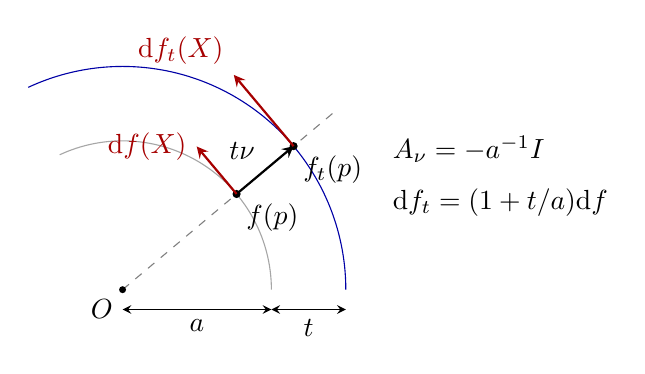
\begin{tikzpicture}[scale=1.05,>=stealth]
	\draw[gray!70] (0:1.8) arc[start angle=0,end angle=115,radius=1.8];
	\draw[blue!65!black] (0:2.7) arc[start angle=0,end angle=115,radius=2.7];
	\draw[gray,dashed] (0,0)--(40:3.35);
	\coordinate (P) at (40:1.8);
	\coordinate (Q) at (40:2.7);
	\fill (0,0) circle (1.2pt) node[below left]{\(O\)};
	\fill (P) circle (1.4pt) node[below right]{\(f(p)\)};
	\fill (Q) circle (1.4pt) node[below right]{\(f_t(p)\)};
	\draw[->,thick] (P)--(Q) node[midway,above left]{\(t\nu\)};
	\draw[->,thick,red!65!black] (P)--++(130:0.75) node[left]{\(\mathrm df(X)\)};
	\draw[->,thick,red!65!black] (Q)--++(130:1.125) node[above left]{\(\mathrm df_t(X)\)};
	\draw[<->] (0,-0.24)--(1.8,-0.24) node[midway,below]{\(a\)};
	\draw[<->] (1.8,-0.24)--(2.7,-0.24) node[midway,below]{\(t\)};
	\node[anchor=west] at (3.15,1.7){\(A_\nu=-a^{-1}I\)};
	\node[anchor=west] at (3.15,1.05){\(\mathrm df_t=(1+t/a)\mathrm df\)};
\end{tikzpicture}

	\caption[圆周的法向偏移]{圆周的外法向偏移。相同角参数的切向微分从内圆移到外圆后放大为原来的 \(1+t/a\) 倍。}
	\label{g3:fig:normal-offset}
\end{figure}

\subsection{超曲面的主曲率}
\label{g3:subsec:0404:02}

余维一时，每个法向值都由一个实数确定。选定单位法向 \(\nu\) 后，写 \(B(X,Y)=g(AX,Y)\nu\)。自伴算子 \(A\) 在每一点有正交单位特征基，其特征值 \(\kappa_1,\ldots,\kappa_n\) 称为该法向下的\term[zhuqulv]{主曲率}[principal curvatures]，相应特征方向称为\term[zhufangxiang]{主方向}[principal directions]。重特征值处未必能把单个主方向光滑选出，下面的逐点公式不需要这种选择。

\begin{proposition}\label{g3:prop:principal-curvature-contractions}
	设 \(f:(M^n,g)\to\bar M^{n+1}\) 是光滑等距浸入，\(n\ge2\)，环境截面曲率恒为 \(c\)。在一点选单位法向 \(\nu\) 及主方向正交单位基 \((e_i)\)，令 \(H_\nu=\langle H,\nu\rangle=n^{-1}\sum_i\kappa_i\)。则
	\begin{align}
		K(e_i,e_j)&=c+\kappa_i\kappa_j\quad(i\ne j),\label{g3:eq:principal-sectional-curvature}\\
		\operatorname{Ric}(e_i,e_j)
		&=\bigl((n-1)c+nH_\nu\kappa_i-\kappa_i^2\bigr)\delta_{ij},\label{g3:eq:principal-ricci-curvature}\\
		\operatorname{Scal}
		&=n(n-1)c+n^2H_\nu^2-|A|^2.\label{g3:eq:hypersurface-scalar-curvature}
	\end{align}
\end{proposition}
\begin{proof}
	Gauss 方程在这组基中成为
	\[
		R_{ijkl}
		=c(\delta_{ik}\delta_{jl}-\delta_{il}\delta_{jk})
		+\kappa_i\kappa_j(\delta_{ik}\delta_{jl}-\delta_{il}\delta_{jk}).
	\]
	取 \(k=i,l=j\) 得到截面公式。固定 \(i\)，把它对 \(j\ne i\) 相加，得到
	\[
		\operatorname{Ric}(e_i,e_i)
		=(n-1)c+\kappa_i\Bigl(\sum_j\kappa_j-\kappa_i\Bigr).
	\]
	非对角分量由同一四阶公式为零。再对 \(i\) 求和，使用 \(|A|^2=\sum_i\kappa_i^2\)，即得标量曲率式。
\end{proof}

这些公式也给出外在形状的限制。例如 Euclid 超曲面若在一点平坦，则 \(\kappa_i\kappa_j=0\) 对所有 \(i\ne j\) 成立，故该点形算子的秩至多为一。若每个截面曲率都严格为正，则任意两个主曲率的乘积均为正，所有主曲率同号。另一方面，全脐点的 \(A=H_\nu I\) 使所有截面曲率等于 \(c+H_\nu^2\)。

\ProseParagraphBreak

法向偏移的主曲率可由式\eqref{g3:eq:parallel-hypersurface-shape}逐个读取：
\[
	\kappa_i(t)=\frac{\kappa_i}{1-t\kappa_i}.
\]
当某个 \(1-t\kappa_i\) 为零时，相应切向方向被 \(\mathrm df_t\) 压为零，偏移参数化失去浸入性。这是一个局部微分条件。即使这些因子都非零，不同基点的法线仍可能在远处相交，因此共同管状半径还需要控制整体单射性。

\subsection{内在曲率相同而外在几何不同}
\label{g3:subsec:0404:03}

内在度量记录沿子流形测量的长度，第二基本形式则记录切空间在环境中的转动。同一度量可以对应不同的第二基本形式；局部基本定理的唯一性因而需要完整的相容数据。

\begin{example}\label{g3:exm:plane-cylinder-isometry}
	在一个平面开矩形 \(U\subset\mathbb R^2\) 上，考虑
	\[
		f_0(u,v)=(u,v,0),\qquad
		f_a(u,v)=\bigl(a\cos(u/a),a\sin(u/a),v\bigr),\quad a>0.
	\]
	两者的诱导度量都是 \(\mathrm du^2+\mathrm dv^2\)，所以具有相同的内在距离局部结构和零 Gauss 曲率。对圆柱取外法向
	\[
		\nu(u,v)=\bigl(\cos(u/a),\sin(u/a),0\bigr),
	\]
	则 \(A_\nu\partial_u=-a^{-1}\partial_u\)、\(A_\nu\partial_v=0\)，而平面上 \(B=0\)。故两者不可能在任何开集上由一个 Euclid 刚性运动联系：环境等距保持第二基本形式，尤其保持其范数。这里一个范数为零，另一个为 \(a^{-1}\)。

	若允许 \(u\) 遍历整个实轴，\(f_a(u+2\pi a,v)=f_a(u,v)\)。因此这个局部等距参数化在整个平面上不单射；把参数域限制到适当的小矩形后，才得到到一块圆柱面的等距微分同胚。
\end{example}

上述区别在高余维中还包括法联络。即使给定相同的 \(g\) 和对称型的分量，换法标架时也必须同时按同一个丛等距变换法联络与 \(B\)。三组相容方程正是对这套几何数据的条件；只比较一张矩阵或只比较内在曲率，不能使用基本定理的唯一性结论。

\subsection{后续面积变分所需的公式}
\label{g3:subsec:0404:04}

当浸入随参数移动时，切向速度主要改变参数点的分布，法向速度才直接与平均曲率配对。先计算诱导度量及其体积密度的导数，便能在任意维数、任意余维得到面积的一阶公式。这里“面积”指 \(n\) 维诱导体积；对非单射浸入按参数流形积分，保留重数。

\begin{theorem}[面积的一阶变分]\label{g3:thm:first-variation-submanifold-area}
	设 \(F:(-\varepsilon,\varepsilon)\times M^n\to(\bar M,\bar g)\) 光滑，每个 \(f_t=F(t,\cdot)\) 都是浸入，\(n\ge1\)。记 \(g_t=f_t^*\bar g\)、\(g=g_0\)，并将初速度分解为 \(V=\partial_tF|_0=\mathrm df_0(W)+V^\perp\)。则
	\begin{align}
		\dot g_0(X,Y)
		&=g(\nabla_XW,Y)+g(X,\nabla_YW)
		-2\langle B(X,Y),V^\perp\rangle,\label{g3:eq:variation-induced-metric}\\
		\left.\frac{\mathrm d}{\mathrm dt}\right|_0\mu_{g_t}
		&=\bigl(\operatorname{div}_gW-n\langle H,V^\perp\rangle\bigr)\mu_g.\label{g3:eq:variation-induced-density}
	\end{align}
	若 \(\Omega\subset M\) 是具有光滑边界的紧区域，\(\eta\) 是 \(\partial\Omega\) 在 \(M\) 内的外单位法向，则
	\begin{equation}\label{g3:eq:first-variation-area-integral}
		\left.\frac{\mathrm d}{\mathrm dt}\right|_0\operatorname{Vol}_{g_t}(\Omega)
		=\int_{\partial\Omega}g(W,\eta)\mu_{\partial g}
		-n\int_\Omega\langle H,V^\perp\rangle\mu_g.
	\end{equation}
\end{theorem}
\begin{proof}
	把 \(X,Y\) 延拓成与时间无关的参数向量场。环境联络度量相容且无挠，因而沿二参数坐标面有 \(\bar\nabla_t\mathrm df_t(X)=\bar\nabla_X\partial_tF\)。逐项求导得到
	\[
		\dot g_0(X,Y)
		=\langle\bar\nabla_XV,\mathrm df_0(Y)\rangle
		+\langle\mathrm df_0(X),\bar\nabla_YV\rangle.
	\]
	代入 \(V=\mathrm df_0(W)+V^\perp\)，用 Gauss 分解和 Weingarten 公式提取切向分量，便得度量变化式。

	在任一固定坐标中，密度系数为 \(\sqrt{\det g_t}\)。可逆矩阵的行列式求导给出
	\[
		\left.\frac{\mathrm d}{\mathrm dt}\right|_0\sqrt{\det g_t}
		=\frac12\operatorname{tr}_g(\dot g_0)\sqrt{\det g}.
	\]
	在一点取正交单位基求迹，前两项各贡献 \(\operatorname{div}_gW\)，最后一项贡献 \(-2n\langle H,V^\perp\rangle\)。这证明密度公式。紧区域上可在积分号下求导，再对 \(W\) 使用\cref{g3:thm:divergence-theorem}，得到边界通量。密度与该散度定理均不要求 \(M\) 可定向。
\end{proof}

\begin{corollary}\label{g3:cor:minimal-area-stationarity}
	设 \(f:M^n\to\bar M\) 为光滑浸入，\(n\ge1\)，\(M\) 无边界。则 \(H=0\) 当且仅当对于任意具有光滑边界的紧区域 \(\Omega\subset M\)，以及任意满足 \(\operatorname{supp}V\subset\operatorname{int}\Omega\) 的上述光滑变分，都有 \(\left.\frac{\mathrm d}{\mathrm dt}\right|_0\operatorname{Vol}_{g_t}(\Omega)=0\)。
\end{corollary}
\begin{proof}
	若 \(H=0\)，在包含初速度支集的紧区域上应用式\eqref{g3:eq:first-variation-area-integral}，边界项和内部项都为零。反过来，若某点 \(H\ne0\)，在其附近选一个非负光滑截断函数 \(\chi\)，支集紧含于一个坐标片，且在该点附近为正。取法向初速度 \(V=\chi H\)。它可以由变分
	\[
		f_t(p)=\exp^{\bar g}_{f(p)}(tV(p))
	\]
	实现：支集紧使共同的小时间可用，指数映射的联合光滑性见\cref{g3:prop:exponential-local}；浸入性是开条件，在这个紧支集上缩小时间便仍成立，支集外则保持原映射。此时一阶变分为 \(-n\int\chi|H|^2\mu_g<0\)，与驻定性矛盾。因此 \(H\) 必处处为零。
\end{proof}

这一结论说明“极小”的一阶意义是面积驻定。是否在所有邻近变分下取得局部最小值，还需要二阶变化的信息。球面外移的检验则直接固定本章符号：若 \(V=\nu\)、\(H=-\nu/a\)，密度导数为 \(n\mu_g/a>0\)，与半径增大一致。

\begin{proposition}\label{g3:prop:immersion-position-laplacian}
	设 \(f:(M^n,g)\to\mathbb R^{n+r}\) 为光滑等距浸入，\(n\ge1\)，对位置向量的各坐标分别使用 \(\Delta_g=-\operatorname{div}_g\operatorname{grad}_g\)。则
	\begin{equation}\label{g3:eq:position-laplacian}
		\Delta_g f=-nH,\qquad
		\Delta_g|f|^2=-2n-2n\langle f,H\rangle.
	\end{equation}
	若像位于 \(S^{n+r-1}(a)\)，以 \(H^S\) 表示相对于球面的平均曲率向量，则
	\begin{equation}\label{g3:eq:spherical-minimal-eigenmap}
		H^{\mathbb R}=H^S-\frac f{a^2},\qquad
		H^S=0\ \Longleftrightarrow\ \Delta_g f=\frac n{a^2}f.
	\end{equation}
\end{proposition}
\begin{proof}
	对任一坐标函数 \(f^\alpha\)，Hessian 的定义给出
	\[
		H_{f^\alpha}(X,Y)
		=\bigl(\mathrm D_X\mathrm df(Y)-\mathrm df(\nabla_XY)\bigr)^\alpha
		=B(X,Y)^\alpha.
	\]
	取负迹即得 \(\Delta_g f=-nH\)。由乘积法则，
	\[
		\Delta_g|f|^2=2\langle f,\Delta_g f\rangle-2|\mathrm df|^2.
	\]
	等距浸入使 \(|\mathrm df|^2=n\)，故得第二式。若像在半径 \(a\) 的球面内，先将环境导数投影到球面的切空间，再投影到 \(M\) 的切空间；球面自身的第二基本形式为 \(-g f/a^2\)。于是
	\[
		B^{\mathbb R}(X,Y)=B^S(X,Y)-\frac{g(X,Y)}{a^2}f.
	\]
	取平均迹得到两个平均曲率的关系，再代入位置向量的 Laplace 公式，便得最后的等价式。
\end{proof}

\begin{corollary}\label{g3:cor:no-compact-euclidean-minimal}
	正维紧无边界光滑流形不存在到 Euclid 空间的极小浸入。
\end{corollary}
\begin{proof}
	若有这样的浸入，以诱导度量计算，由 \(H=0\) 及式\eqref{g3:eq:position-laplacian}，有 \(\Delta_g|f|^2=-2n\)。在 \(M\) 上积分，散度定理使左边为零，右边却是 \(-2n\operatorname{Vol}_g(M)<0\)，矛盾。
\end{proof}

球面中的极小乘积没有这一矛盾：其 Euclid 平均曲率为 \(-f/a^2\)，在位置向量公式中恰好抵消常数项。这样，局部的切法分解、相容方程及整体积分在同一个模型上相互核对。


\begin{chaptersummary}
	切向与法向投影把环境导数分成内在 Levi-Civita 联络、第二基本形式、形算子及法联络。第二基本形式的对称性来自无挠性，形算子是它与指定法向配对后的自伴算子，平均曲率向量则是其平均迹。高余维法空间的变化具有自己的曲率，不能由单个形算子代替。

	\ProseParagraphBreak

	Gauss、Codazzi 和 Ricci 方程分别比较切曲率、第二基本形式的导数与法曲率。在空间形式中，它们恰好使所构造的切法直和联络或其增广联络平坦。积分平坦标架，再积分位置数据，就得到局部浸入；同一数据的两次构造相差环境等距。整体实现还要求沿闭路的标架返回以及 Euclid 情形的位置周期相容，局部方程本身不会消去这些障碍。

	\ProseParagraphBreak

	模型计算展示了内在和外在信息的不同作用：平面与圆柱可以局部等距，球面乘积可以在球面内极小而在 Euclid 空间中不极小，法向偏移的正则性则由形算子的特征值控制。面积的一阶变化由边界通量与平均曲率配对给出；无边界紧支变分下，\(H=0\) 等价于面积驻定。位置向量的 Laplace 公式进一步把这一外在条件转化为可积分的函数等式。
\end{chaptersummary}

\BookExercises

\begin{exercise}\label{g3:ex:graph-prescribed-second-fundamental-form}
	设 \(h:U\to\mathbb R^r\) 光滑，其中 \(U\subset\mathbb R^n\) 为原点邻域，\(n\ge1\)，且 \(h(0)=0\)、\(\mathrm dh_0=0\)。考虑图像浸入
	\[
		f(x)=(x,h(x))\in\mathbb R^{n+r},
	\]
	并给 \(U\) 诱导度量。
	\begin{enumerate}
		\item 求原点处的度量、联络系数、第二基本形式及平均曲率向量。将形算子写成 \(h\) 的二阶偏导矩阵。
		\item 给定任意对称双线性映射 \(C:\mathbb R^n\times\mathbb R^n\to\mathbb R^r\)，构造一个这样的图像，使其原点第二基本形式等于 \(C\)。当 \(n\ge2\)、\(r\ge1\) 时，给出 \(H(0)=0\) 而 \(B_0\ne0\) 的具体例子。
	\end{enumerate}
\end{exercise}
\begin{solution}
	1. 记 \(h_i^\alpha=\partial_i h^\alpha\)。坐标切向量及度量为
	\[
		f_i=(e_i,h_i),\qquad
		g_{ij}=\delta_{ij}+\sum_{\alpha=1}^r h_i^\alpha h_j^\alpha.
	\]
	因为 \(h_i^\alpha(0)=0\)，有 \(g_{ij}(0)=\delta_{ij}\)，且
	\[
		\partial_kg_{ij}(0)
		=\sum_\alpha
			\bigl(h_{ik}^\alpha h_j^\alpha+h_i^\alpha h_{jk}^\alpha\bigr)(0)=0.
	\]
	由 Christoffel 公式，\(\Gamma^k_{ij}(0)=0\)。原点切空间是水平的 \(\mathbb R^n\times\{0\}\)，法空间是竖直的 \(\{0\}\times\mathbb R^r\)，而
	\[
		\partial_i\partial_jf(0)
		=\left(0,\bigl(\partial_i\partial_jh^\alpha(0)\bigr)_{\alpha=1}^r\right)
	\]
	已经法向。因此
	\[
		B_0(e_i,e_j)
		=\left(0,\bigl(\partial_i\partial_jh^\alpha(0)\bigr)_\alpha\right),
		\qquad
		H(0)=\frac1n
			\left(0,\bigl(\sum_i\partial_i^2h^\alpha(0)\bigr)_\alpha\right).
	\]
	对法向量 \(\xi=(0,\xi^1,\ldots,\xi^r)\)，形算子在水平正交基中的矩阵为
	\[
		(A_\xi)_{ij}
		=\sum_{\alpha=1}^r\xi^\alpha\partial_i\partial_jh^\alpha(0).
	\]
	矩阵对称，对应 \(B\) 的对称性。这里原点处 \(\partial g=0\) 已足以计算联络与 \(B\)，不需要把整个图像坐标识别为法坐标。

	2. 写 \(C(e_i,e_j)=C_{ij}\in\mathbb R^r\)，并取
	\[
		h(x)=\frac12C(x,x)=\frac12\sum_{i,j}C_{ij}x^ix^j.
	\]
	对称性给出 \(\partial_i\partial_jh=C_{ij}\)，且 \(h(0)=0\)、\(\mathrm dh_0=0\)。图像的前 \(n\) 个分量就是 \(x\)，所以处处为浸入；第 1 问表明其原点第二基本形式恰为给定的 \(C\)。

	当 \(n\ge2\)、\(r\ge1\) 时，取
	\[
		h^1(x)=\frac12\bigl((x^1)^2-(x^2)^2\bigr),\qquad
		h^\alpha(x)=0\quad(\alpha>1).
	\]
	记 \(\varepsilon_1\) 为 \(\mathbb R^r\) 的第一个标准基向量。原点处 \(B(e_1,e_1)=(0,\varepsilon_1)\)、\(B(e_2,e_2)=-(0,\varepsilon_1)\)，其他对角分量为零，因此 \(H(0)=0\)，但 \(B_0\ne0\)。这显示一点处平均曲率为零允许不同切向方向的法向弯曲相互抵消。
\end{solution}

\begin{exercise}\label{g3:ex:normal-frame-change}
	设 \(f:(M,g)\to(\bar M,\bar g)\) 为光滑等距浸入，在开集 \(U\subset M\) 上取正交单位法标架 \(\nu=(\nu_1,\ldots,\nu_r)\)，写
	\(\nabla^\perp\nu=\nu\eta\)、\(F^\perp=\mathrm d\eta+\eta\wedge\eta\)。
	\begin{enumerate}
		\item 若 \(\nu'=\nu Q\)，其中 \(Q:U\to\operatorname{O}(r)\) 光滑，证明
		\[
			\eta'=Q^{-1}\eta Q+Q^{-1}\mathrm dQ,\qquad
			(F^\perp)'=Q^{-1}F^\perp Q.
		\]
		\item 设法丛秩为二，在定向正交单位法标架中写
		\[
			\eta=\begin{pmatrix}0&-\alpha\\\alpha&0\end{pmatrix}.
		\]
		若 \(Q\) 为角度 \(\phi\) 的转动矩阵，求 \(\alpha'\)。进一步，若 \(U\) 是二维坐标矩形，证明在 \(U\) 上存在由这种转动得到的法平行标架，当且仅当 \(\mathrm d\alpha=0\)。充分性中直接构造 \(\phi\)。
	\end{enumerate}
\end{exercise}
\begin{solution}
	1. 联络的乘积规则给出
	\[
		\nabla^\perp(\nu Q)=\nu(\eta Q+\mathrm dQ)
		=\nu Q\bigl(Q^{-1}\eta Q+Q^{-1}\mathrm dQ\bigr),
	\]
	所以括号中就是新标架的联络矩阵。曲率对法向输入为函数线性，故
	\[
		R^\perp(X,Y)(\nu Q)=\nu F^\perp(X,Y)Q
		=\nu Q\bigl(Q^{-1}F^\perp(X,Y)Q\bigr).
	\]
	这证明曲率矩阵按共轭变换，并由此再见 \(R^\perp\) 是否为零与标架无关。

	2. 记
	\[
		J=\begin{pmatrix}0&-1\\1&0\end{pmatrix},\qquad
		Q=\begin{pmatrix}\cos\phi&-\sin\phi\\
			\sin\phi&\cos\phi\end{pmatrix}.
	\]
	\(JQ=QJ\)，且 \(Q^{-1}\mathrm dQ=J\,\mathrm d\phi\)，所以
	\[
		\eta'=J(\alpha+\mathrm d\phi),\qquad
		\alpha'=\alpha+\mathrm d\phi.
	\]
	又因 \(\alpha\wedge\alpha=0\)，有 \(F^\perp=J\,\mathrm d\alpha\)。若转动后标架法平行，则 \(\alpha'=0\)，从而 \(\mathrm d\alpha=0\)。

	反过来，在坐标矩形上写 \(\alpha=a(x,y)\,\mathrm dx+b(x,y)\,\mathrm dy\)，并固定其中一点 \((x_0,y_0)\)。闭性意味着 \(\partial_xb=\partial_ya\)。令
	\[
		\phi(x,y)
		=-\int_{x_0}^x a(t,y_0)\,\mathrm dt
			-\int_{y_0}^y b(x,s)\,\mathrm ds.
	\]
	矩形保证两段积分道路都在坐标域内。直接求导，
	\[
		\partial_y\phi=-b(x,y),\qquad
		\partial_x\phi=-a(x,y_0)
			-\int_{y_0}^y\partial_xb(x,s)\,\mathrm ds=-a(x,y).
	\]
	故 \(\mathrm d\phi=-\alpha\)，从而 \(\alpha'=0\)，所得正交单位法标架处处法平行。矩形条件在这里提供了单值的原函数构造；只有一点处曲率为零，并不足以使这一构造适用于整个邻域。
\end{solution}

\begin{exercise}\label{g3:ex:helix-normal-parallel-frame}
	设 \(a>0\)、\(b\ne0\)、\(c=\sqrt{a^2+b^2}\)，考虑 Euclid 空间中的单位速曲线
	\[
		\gamma(s)=\left(a\cos\frac sc,\ a\sin\frac sc,\ \frac bc s\right),
		\qquad s\in\mathbb R.
	\]
	记 \(T=\gamma'\)，并定义
	\[
		\nu_1(s)=\left(-\cos\frac sc,-\sin\frac sc,0\right),\qquad
		\nu_2(s)=\left(\frac bc\sin\frac sc,-\frac bc\cos\frac sc,\frac ac\right).
	\]
	\begin{enumerate}
		\item 验证 \((T,\nu_1,\nu_2)\) 为正交单位标架，求第二基本形式、平均曲率向量及法联络矩阵。
		\item 构造整个参数直线上的正交单位法平行标架。说明法平行不等于作为 \(\mathbb R^3\) 中的向量保持不变。
		\item 证明此曲线的法联络曲率为零，但其平均曲率向量不法平行，虽然 \(|H|\) 为常数。
	\end{enumerate}
\end{exercise}
\begin{solution}
	1. 求导得到
	\[
		T=\left(-\frac ac\sin\frac sc,\frac ac\cos\frac sc,\frac bc\right).
	\]
	由 \(a^2+b^2=c^2\)，三个向量的长度都为一，互相内积为零。令
	\[
		\kappa=\frac a{c^2},\qquad \tau=\frac b{c^2}.
	\]
	直接求导并在此标架中分解，得到
	\[
		T'=\kappa\nu_1,\qquad
		\nu_1'=-\kappa T+\tau\nu_2,\qquad
		\nu_2'=-\tau\nu_1.
	\]
	参数直线取诱导度量 \(\mathrm ds^2\)。于是
	\[
		B(\partial_s,\partial_s)=H=\kappa\nu_1,\qquad
		\nabla^\perp_{\partial_s}\nu_1=\tau\nu_2,\qquad
		\nabla^\perp_{\partial_s}\nu_2=-\tau\nu_1.
	\]
	行标架 \(\nu=(\nu_1,\nu_2)\) 的法联络矩阵为
	\[
		\eta=\begin{pmatrix}0&-\tau\\\tau&0\end{pmatrix}\mathrm ds.
	\]

	2. 取转动角 \(\phi(s)=-\tau s\)，并令
	\[
		\begin{aligned}
			E_1&=\cos(\tau s)\nu_1-\sin(\tau s)\nu_2,\\
			E_2&=\sin(\tau s)\nu_1+\cos(\tau s)\nu_2.
		\end{aligned}
	\]
	这是处处正交的转动，所以 \((E_1,E_2)\) 仍为正交单位法标架。利用第 1 问的导数式，各个法向项逐对抵消，得到
	\[
		E_1'=-\kappa\cos(\tau s)T,\qquad
		E_2'=-\kappa\sin(\tau s)T.
	\]
	两个导数都切向，故 \(\nabla^\perp_{\partial_s}E_1=
	\nabla^\perp_{\partial_s}E_2=0\)。但 \(E_1'(0)=-\kappa T(0)\ne0\)，所以法平行向量场仍可以作为环境向量改变；改变的部分恰好全部切向。

	3. 法曲率对两个切向输入反对称，一维切空间中任意两个输入线性相关，故 \(R^\perp=0\)。在给定标架中也可直接计算：\(\mathrm d\eta=0\)，且 \(\eta\wedge\eta\) 含因子 \(\mathrm ds\wedge\mathrm ds=0\)。另一方面，
	\[
		|H|=\kappa,\qquad
		\nabla^\perp_{\partial_s}H
		=\kappa\tau\nu_2\ne0,
	\]
	因为 \(\kappa>0\)、\(\tau\ne0\)。法联络平坦、某个法向场长度恒定、该法向场法平行，是三个不同的条件。
\end{solution}

% 第三卷第四章习题草稿：一般余维收缩、极小浸入、二维法曲率。
% 合入章文件后由章内环境连续编号。

\begin{exercise}\label{g3:ex:submanifold-ricci-scalar-contractions}
	设 \(F\colon(M^n,g)\to\bar M^{n+q}\) 为到常截面曲率 \(c\) 空间的光滑等距浸入，\(n\ge2\)。令 \(B\) 为第二基本形式，\(H=\operatorname{tr}_gB/n\)，并对任一正交单位基 \((e_i)\) 定义
	\[
		\lVert B\rVert^2=\sum_{i,j}\lVert B(e_i,e_j)\rVert^2,
		\qquad B^\circ(X,Y)=B(X,Y)-g(X,Y)H.
	\]
	由 Gauss 方程求 \(\operatorname{Ric}\) 与 \(\operatorname{Scal}\) 的一般余维表达式，证明
	\[
		\operatorname{Scal}\le n(n-1)(c+\lVert H\rVert^2),
	\]
	并用 \(B^\circ\) 描述逐点取等的充要条件。最后说明最小维数 \(n=2\) 时所得不等式的几何含义。
\end{exercise}
\begin{solution}
	固定一点，并在该点取正交单位基 \((e_i)\)。按照本卷的曲率次序，\(\operatorname{Ric}(X,Y)=\sum_i\mathrm{Rm}(e_i,X,e_i,Y)\)。对 \eqref{g3:eq:gauss-space-form} 收缩，环境项为
	\[
		c\sum_i\bigl(g(X,Y)-g(e_i,Y)g(X,e_i)\bigr)
		=(n-1)c\,g(X,Y).
	\]
	第二基本形式的两个项分别给出
	\[
		\sum_i\langle B(e_i,e_i),B(X,Y)\rangle
		=n\langle H,B(X,Y)\rangle,
	\]
	以及 \(-\sum_i\langle B(X,e_i),B(Y,e_i)\rangle\)。因此
	\[
		\operatorname{Ric}(X,Y)
		=(n-1)c\,g(X,Y)+n\langle H,B(X,Y)\rangle
		-\sum_i\langle B(X,e_i),B(Y,e_i)\rangle.
	\]
	再取迹得到
	\[
		\operatorname{Scal}
		=n(n-1)c+n^2\lVert H\rVert^2-\lVert B\rVert^2.
	\]
	以上均为张量的度量收缩，所以不依赖所取正交单位基。

	展开无迹部分的平方，利用 \(\sum_iB(e_i,e_i)=nH\)，有
	\[
		\begin{aligned}
		\lVert B^\circ\rVert^2
		&=\sum_{i,j}\lVert B(e_i,e_j)-\delta_{ij}H\rVert^2\\
		&=\lVert B\rVert^2-2\sum_i\langle B(e_i,e_i),H\rangle
		+n\lVert H\rVert^2\\
		&=\lVert B\rVert^2-n\lVert H\rVert^2.
		\end{aligned}
	\]
	于是精确的差值是
	\[
		\operatorname{Scal}
		=n(n-1)(c+\lVert H\rVert^2)-\lVert B^\circ\rVert^2.
	\]
	范数平方非负给出题设不等式，且某点取等当且仅当 \(B^\circ=0\)，即该点满足 \(B(X,Y)=g(X,Y)H\)，正是脐点条件。当 \(n=2\) 时，\(\operatorname{Scal}=2K\)，所以
	\[
		K=c+\lVert H\rVert^2-\tfrac12\lVert B^\circ\rVert^2
		\le c+\lVert H\rVert^2.
	\]
	因此在环境曲率和平均曲率向量给定时，偏离脐性的部分精确降低了内在 Gauss 曲率。
\end{solution}

\begin{exercise}\label{g3:ex:minimal-euclidean-ricci-nullity}
	设 \(F\colon(M^n,g)\to\mathbb R^{n+q}\) 为光滑极小等距浸入，即 \(H=0\)。证明 \(\operatorname{Ric}\) 为半负定，并求出其作为双线性型的核
	\[
		\ker\operatorname{Ric}_p
		=\{v\in\mathrm{T}_pM:\operatorname{Ric}_p(v,w)=0
		\text{ 对每个 }w\in\mathrm{T}_pM\}.
	\]
	进一步证明 \(\operatorname{Ric}_p=0\) 当且仅当 \(B_p=0\)，并推出：若一个极小 Euclid 浸入的诱导度量平直，则它全测地。解释为何删除极小性后最后一个结论不再成立。
\end{exercise}
\begin{solution}
	由上一题的 Ricci 收缩公式，令 \(c=0\)、\(H=0\)，便有
	\[
		\operatorname{Ric}_p(v,w)
		=-\sum_i\langle B_p(v,e_i),B_p(w,e_i)\rangle.
	\]
	特别地，\(\operatorname{Ric}_p(v,v)=-\sum_i\lVert B_p(v,e_i)\rVert^2\le0\)。如果 \(v\) 属于 Ricci 型的核，取 \(w=v\) 可知每个 \(B_p(v,e_i)\) 都为零，故由线性性 \(B_p(v,w)=0\) 对任意 \(w\) 成立。反过来，若这一条件成立，所显示的双线性公式立即给出 \(v\in\ker\operatorname{Ric}_p\)。因此
	\[
		\ker\operatorname{Ric}_p
		=\{v\in\mathrm{T}_pM:B_p(v,w)=0\text{ 对所有 }w\in\mathrm{T}_pM\}.
	\]
	若 \(\operatorname{Ric}_p=0\)，上述核就是整个切空间，所以 \(B_p=0\)；反向蕴含也由同一公式得到。

	若诱导度量平直，则每点的 Ricci 张量为零，因而 \(B=0\)。由 \cref{g3:prop:totally-geodesic-characterization}，浸入全测地。这里用到了极小性：例如半径为 \(a>0\) 的圆柱
	\[
		F(s,t)=(a\cos(s/a),a\sin(s/a),t)
	\]
	诱导度量为 \(\mathrm ds^2+\mathrm dt^2\)，但采用外法向时，\(B(\partial_s,\partial_s)=-\nu/a\)、\(B(\partial_t,\partial_t)=B(\partial_s,\partial_t)=0\)，所以 \(B\ne0\) 且 \(H=-\nu/(2a)\ne0\)。平直性本身不排除这种弯曲。
\end{solution}

\begin{exercise}\label{g3:ex:minimal-surface-normal-curvature-bound}
	设 \(F\colon M^2\to\mathbb R^4\) 为光滑极小等距浸入，在一点 \(p\) 选取切空间和法空间的正交单位基 \((e_1,e_2)\)、\((\nu_1,\nu_2)\)。由于极小性，可写
	\[
		A_{\nu_1}=\begin{pmatrix}a&b\\b&-a\end{pmatrix},
		\qquad
		A_{\nu_2}=\begin{pmatrix}c&d\\d&-c\end{pmatrix}.
	\]
	记 \(K\) 为内在 Gauss 曲率，并相对于所选两组基定义
	\[
		K^\perp=\langle R^\perp(e_1,e_2)\nu_1,\nu_2\rangle.
	\]
	计算 \(K\) 与 \(K^\perp\)，证明 \(\lvert K^\perp\rvert\le-K\)，并给出取等条件。将等号条件解释为法平面内曲线
	\[
		\theta\longmapsto
		B(\cos\theta\,e_1+\sin\theta\,e_2,
		  \cos\theta\,e_1+\sin\theta\,e_2)
	\]
	的几何性质，允许该曲线退化为一点。
\end{exercise}
\begin{solution}
	把法平面用所选基识别为 \(\mathbb R^2\)，则
	\[
		u\coloneqq B(e_1,e_1)=(a,c),\qquad
		v\coloneqq B(e_1,e_2)=(b,d),\qquad
		B(e_2,e_2)=-u.
	\]
	Gauss 方程给出
	\[
		K=-\lVert u\rVert^2-\lVert v\rVert^2
		=-(a^2+b^2+c^2+d^2).
	\]
	Ricci 方程则给出 \(K^\perp=g([A_{\nu_1},A_{\nu_2}]e_1,e_2)\)。直接相乘有
	\[
		[A_{\nu_1},A_{\nu_2}]
		=\begin{pmatrix}0&2(ad-bc)\\2(bc-ad)&0\end{pmatrix},
	\]
	所以在本卷的符号约定下，
	\[
		K^\perp=2(bc-ad)=-2\det(u,v).
	\]
	反转任一组基的定向会改变 \(K^\perp\) 的符号，但不影响下面的绝对值不等式。利用平面行列式的估计和平方差，有
	\[
		\lvert K^\perp\rvert
		=2\lvert\det(u,v)\rvert
		\le2\lVert u\rVert\lVert v\rVert
		\le\lVert u\rVert^2+\lVert v\rVert^2=-K.
	\]
	两步同时取等当且仅当 \(u\perp v\) 且 \(\lVert u\rVert=\lVert v\rVert\)，其中包括 \(u=v=0\)。用矩阵分量写为
	\[
		ab+cd=0,\qquad a^2+c^2=b^2+d^2.
	\]
	最后利用双线性和 \(B(e_2,e_2)=-u\)，题设曲线为
	\[
		u\cos(2\theta)+v\sin(2\theta).
	\]
	它是单位圆在以 \(u,v\) 为列向量的线性映射下的像，通常为椭圆。若 \(u,v\) 正交且等长，则其像为以原点为圆心的圆；两者都为零时退化为原点。反过来，若此像是半径 \(\rho>0\) 的圆，则在 \(2\theta=0,\pi/2,\pi/4\) 处比较到原点的距离，先得 \(\lVert u\rVert=\lVert v\rVert=\rho\)，再得 \(\langle u,v\rangle=0\)。退化为一点时，其中心为原点且 \(u=v=0\)。故题设不等式取等恰好对应这一个圆形或点形的情形。
\end{solution}

\begin{exercise}\label{g3:ex:normal-data-gauge-equivalence}
	设 \((M,g)\) 为无边界光滑黎曼流形，\(E,E'\to M\) 为同秩光滑 Euclid 向量丛，\(J:E\to E'\) 是覆盖恒等映射的光滑纤维等距。给定 \(E\) 上的度量联络 \(\nabla^E\) 与对称型 \(B\)，在 \(E'\) 上定义
	\[
		B'(X,Y)=J B(X,Y),\qquad
		\nabla^{E'}_X\xi'=J\bigl(\nabla^E_X(J^{-1}\xi')\bigr).
	\]
	\begin{enumerate}
		\item 证明新旧数据同时满足给定 \(c\) 的三组相容方程，并求两个数据联络之间的关系。
		\item 若 \((f,\iota)\) 实现原数据，写出实现新数据的同一个浸入的法丛识别。说明为什么旋转法标架时不能只旋转 \(B\) 的分量而保持联络矩阵不变。
	\end{enumerate}
\end{exercise}
\begin{solution}
	1. 由定义及 \(J\) 保持内积，\(\nabla^{E'}\) 满足联络的乘积规则并保持新内积。对 \(\xi\in\Gamma(E)\)，形算子满足
	\[
		g(A'_{J\xi}X,Y)
		=\langle JB(X,Y),J\xi\rangle_{E'}
		=g(A_\xi X,Y),
	\]
	所以 \(A'_{J\xi}=A_\xi\)。连续使用两次联络定义，得到
	\[
		R^{E'}(X,Y)(J\xi)=J(R^E(X,Y)\xi),
		\qquad(\nabla B')(X;Y,Z)=J((\nabla B)(X;Y,Z)).
	\]
	Gauss 式中的内积不变，Codazzi 的两边同乘 \(J\)，Ricci 式的两边也由上述曲率与形算子关系保持。因此相容性等价。

	令 \(L=\operatorname{id}_{\mathrm TM}\oplus J\)。对式\eqref{g3:eq:submanifold-data-connection}逐项代入，得到
	\[
		D'_X(L\sigma)=L(D_X\sigma).
	\]
	若 \(c\ne0\)，把 \(L\) 扩充为在 \(s\) 上取恒等，同样有 \(\widehat D'_XL=L\widehat D_X\)。所以两个数据联络只是经同一个纤维等距识别后的同一联络；平坦性及沿闭路径的返回条件同时成立。

	2. 取 \(\iota'=\iota\circ J^{-1}\)。则
	\[
		\iota'B'=\iota B=B_f,
		\qquad
		\nabla^{\perp,f}_X(\iota'\xi')
		=\iota'(\nabla^{E'}_X\xi'),
	\]
	故 \((f,\iota')\) 实现新数据。

	再用矩阵说明旋转标架的影响。设 \(\nu\) 是同一个法丛中的行正交标架，\(\nabla^E\nu=\nu\omega\)，并换为 \(\nu'=\nu O\)，其中 \(O:M\to\operatorname O(r)\) 光滑。由乘积规则，
	\[
		\omega'=O^{-1}\omega O+O^{-1}\mathrm dO.
	\]
	若 \(B=\nu b\)，其新分量为 \(b'=O^{-1}b\)。额外的 \(O^{-1}\mathrm dO\) 记录法标架自身的变化，必须与 \(B\) 分量的变化同时计入。例如在区间上，原联络矩阵为零，取
	\[
		O(s)=\begin{pmatrix}\cos s&-\sin s\\ \sin s&\cos s\end{pmatrix},
	\]
	则新矩阵为 \(\left(\begin{smallmatrix}0&-1\\1&0\end{smallmatrix}\right)\mathrm ds\)，并不为零。把它强行保持为零，会换掉法联络，因而改变给定的几何数据。
\end{solution}

\begin{exercise}\label{g3:ex:fundamental-theorem-smooth-families}
	设 \(U_0\subset\mathbb R^n\) 是含原点的开集，\(\lambda\) 属于 \(0\) 的有限维参数邻域。固定 \(c\in\mathbb R\)，在 \(U_0\) 上给定一族数据 \((g_\lambda,E,\langle\ ,\ \rangle_\lambda,\nabla^{E,\lambda},B_\lambda)\)，其中 \(E=U_0\times\mathbb R^r\)，所有局部分量对 \((x,\lambda)\) 联合光滑，各纤维内积正定，每组数据都满足曲率 \(c\) 的相容方程。
	\begin{enumerate}
		\item 在原点给定光滑依赖 \(\lambda\) 的初始线性等距：\(c=0\) 时从 \((\mathrm TM\oplus E)_0\) 到 \(\mathbb R^{n+r}\)，\(c\ne0\) 时从增广纤维 \((\mathrm TM\oplus E\oplus\mathbb Rs)_0\) 到相应的线性环境空间。Euclid 情形再给定光滑的初始位置；\(c<0\) 时要求初始等距将 \(s_0\) 送到最后一坐标为正的单位向量。证明缩小坐标域与参数域后，可以选择实现 \((f_\lambda,\iota_\lambda)\) 对 \((x,\lambda)\) 联合光滑，并具有所给初值。
		\item 若 \(\lambda\) 为实参数，且 \(g_\lambda=g\) 不变，令 \(V=\left.\partial_\lambda f_\lambda\right|_{\lambda=0}\)。证明
		\[
			\langle\nabla^{Q}_X V,\mathrm df_0(Y)\rangle
			+\langle\mathrm df_0(X),\nabla^{Q}_Y V\rangle=0.
		\]
		将 \(V=\mathrm df_0(Z)+\eta\) 分成切向与法向后，把这一式子写成 \(Z,\eta,B_{f_0}\) 的关系。
	\end{enumerate}
\end{exercise}
\begin{solution}
	1. 因度量与纤维内积对参数光滑且在原点正定，可在共同小邻域中对固定基作逐次正交归一化；每一步只涉及光滑运算与正数开平方，故所得标架对 \((x,\lambda)\) 联合光滑。相应的 Levi-Civita 联络系数由度量、逆矩阵与一阶导数给出，故也联合光滑。于是式\eqref{g3:eq:submanifold-data-connection}或式\eqref{g3:eq:augmented-submanifold-connection}的所有系数均联合光滑。

	在\cref{g3:lem:flat-connection-local-frame}的逐轴构造中，将 \(\lambda\) 与尚未行进的坐标一起作为参数。常微分方程的光滑依赖给出共同小盒与参数邻域中的光滑解矩阵。构造只有有限个坐标步骤，因此有限次缩小后，所有步骤都有同一个定义域。给定的初始线性等距也光滑依赖参数，所以最终 \(\Phi_\lambda\) 联合光滑。

	若 \(c=0\)，则 \(\alpha_\lambda(X)=\Phi_\lambda(X)\) 联合光滑，在固定区间 \([0,1]\) 上使用式\eqref{g3:eq:star-shaped-one-form-primitive}积分，给出联合光滑的 \(f_\lambda\)。若 \(c\ne0\)，直接取 \(f_\lambda=a^{-1}\Phi_\lambda(s)\)；双曲情形的初始同构取向指定片，缩小后仍在该片内。两种情形都取 \(\iota_\lambda=\Phi_\lambda|_E\)，从而满足全部要求。唯一性由初始标架及位置已经固定得到。

	2. 对 \(f_\lambda^*g_Q=g\) 求参数导数。环境联络保持度量，并且无挠性给出
	\[
		\left.\nabla_{\partial_\lambda}^{Q}\bigl(\mathrm df_\lambda(X)\bigr)\right|_0
		=\nabla_X^{Q}V.
	\]
	这个交换也可在环境坐标中直接检查：二阶普通偏导交换，联络修正项中的系数关于两个下标对称。度量右侧不随参数变化，于是得到题述等式。

	由 Gauss 与 Weingarten 公式，\(\nabla_X^Q V\) 的切向部分为
	\[
		\mathrm df_0(\nabla_XZ-A_\eta X).
	\]
	代入后得到
	\[
		g(\nabla_XZ,Y)+g(X,\nabla_YZ)
		=2\langle B_{f_0}(X,Y),\eta\rangle.
	\]
	这给出保持诱导度量的一阶必要条件：切向变化的对称导数恰好补偿法向变化通过第二基本形式产生的度量变化。此处结论来自已经存在的光滑实现族，并没有断言每个满足这一线性方程的 \(V\) 都能积分成等距浸入族。
\end{solution}

\begin{exercise}\label{g3:ex:closed-curve-data-monodromy}
	设 \(M=\mathbb R/L\mathbb Z\)，\(L>0\)，取度量 \(\mathrm ds^2\) 及单位切向场 \(e=\partial_s\)。令 \(E=M\times\mathbb R^2\) 有全局正交单位标架 \(\nu_1,\nu_2\)，给定常数 \(\kappa>0\)、\(\tau\in\mathbb R\)，规定
	\[
		B(e,e)=\kappa\nu_1,\qquad
		\nabla^E_e\nu_1=\tau\nu_2,\qquad
		\nabla^E_e\nu_2=-\tau\nu_1.
	\]
	\begin{enumerate}
		\item 验证这些数据满足 \(c=0\) 的全部相容方程，并求数据联络 \(D\) 在标架 \((e,\nu_1,\nu_2)\) 中的矩阵。
		\item 令 \(q=\sqrt{\kappa^2+\tau^2}\)。验证参数直线上的曲线
		\[
			f(s)=\left(\frac{\kappa}{q^2}\cos(qs),
			\frac{\kappa}{q^2}\sin(qs),\frac{\tau}{q}s\right)
		\]
		实现提升后的数据。求这些数据在 \(M\) 上存在带所给法丛识别的整体浸入 \(M\to\mathbb R^3\) 的充要条件。
		\item 证明线性标架沿一周返回原值当且仅当 \(qL\in2\pi\mathbb Z\)。说明此条件单独成立为何还不能保证位置闭合。
	\end{enumerate}
\end{exercise}
\begin{solution}
	1. 在一维上，曲率二形式为零，Gauss 与 Codazzi 两边关于最前两个方向反对称，因而均为零。形算子在一维切空间上都是数乘，彼此交换，所以 Ricci 方程也成立。\(A_{\nu_1}e=\kappa e\)、\(A_{\nu_2}e=0\)，数据联络因此满足
	\[
		D_ee=\kappa\nu_1,\quad
		D_e\nu_1=-\kappa e+\tau\nu_2,\quad
		D_e\nu_2=-\tau\nu_1.
	\]
	按行标架、列分量约定，其矩阵为 \(\Omega\,\mathrm ds\)，其中
	\[
		\Omega=\begin{pmatrix}
			0&-\kappa&0\\
			\kappa&0&-\tau\\
			0&\tau&0
		\end{pmatrix}.
	\]

	2. 直接求导，记
	\[
		\begin{aligned}
		T&=f'=\left(-\frac\kappa q\sin(qs),\frac\kappa q\cos(qs),\frac\tau q\right),\\
		N_1&=(-\cos(qs),-\sin(qs),0),\\
		N_2&=\left(\frac\tau q\sin(qs),-\frac\tau q\cos(qs),\frac\kappa q\right).
		\end{aligned}
	\]
	这三向量是正交单位基，并且
	\[
		T'=\kappa N_1,\qquad
		N_1'=-\kappa T+\tau N_2,\qquad
		N_2'=-\tau N_1.
	\]
	取 \(\iota(\nu_i)=N_i\)，即可逐项读出所给的第二基本形式及法联络，故该曲线实现数据。

	若存在圆周上的整体实现，将它沿 \(\mathbb R\to\mathbb R/L\mathbb Z\) 提升到参数直线。\cref{g3:prop:submanifold-fundamental-uniqueness}说明它与上述 \(f\) 只差一个刚性变换，因此必须有 \(f(s+L)=f(s)\)。第三坐标之差为 \(\tau L/q\)，所以必有 \(\tau=0\)。此时 \(q=\kappa\)，前两个坐标周期要求 \(\kappa L\in2\pi\mathbb Z\)。反之，这两个条件成立时，\(f,T,N_1,N_2\) 都为 \(L\) 周期，故曲线和法丛识别同时下降到圆周。因此充要条件为
	\[
		\tau=0,\qquad \kappa L=2\pi m\quad\text{对某个整数 }m\geq1.
	\]
	当 \(m>1\) 时，所得浸入多次绕过同一个圆，其成立并不要求单射。

	3. \(\Omega\) 的核由 \((\tau,0,\kappa)\) 张成；在其正交补上，直接计算得到 \(\Omega^2=-q^2I\)。因此指数 \(\exp(-L\Omega)\) 在核上为恒等，在正交补上是转角大小为 \(qL\) 的平面旋转。这正是平行方程 \(u'=-\Omega u\) 沿一周的解矩阵，故返回为恒等恰当且仅当 \(qL\in2\pi\mathbb Z\)。

	若满足这一条件而 \(\tau\ne0\)，则三向量 \(T,N_1,N_2\) 都已经返回，但
	\[
		f(s+L)-f(s)=\left(0,0,\frac{\tau L}{q}\right)\ne0.
	\]
	标架的旋转障碍已经消失，位置仍有非零平移周期。这个差向量正是式\eqref{g3:eq:euclidean-development-periods}中的闭路径积分，说明必须同时检查两个返回条件。
\end{solution}

\begin{exercise}\label{g3:ex:prescribed-cylinder-bending}
	给定光滑函数 \(k:\mathbb R\to\mathbb R\)，构造光滑等距浸入 \(f:(\mathbb R^2,\mathrm ds^2+\mathrm dz^2)\to\mathbb R^3\)，使它在某个全局单位法向下的形算子为 \(\operatorname{diag}(k(s),0)\)。证明诱导度量完备，并说明当 \(k\) 非常数时，这个浸入为何在内在平坦的同时具有变化的外在曲率。
\end{exercise}
\begin{solution}
	令
	\[
		\theta(s)=\int_0^s k(\tau)\,\mathrm d\tau,\qquad
		\gamma(s)=\left(\int_0^s\cos\theta(\tau)\,\mathrm d\tau,
		\int_0^s\sin\theta(\tau)\,\mathrm d\tau\right).
	\]
	于是 \(\gamma'=(\cos\theta,\sin\theta)\) 为单位向量，且
	\[
		\gamma''=k(s)(-\sin\theta,\cos\theta).
	\]
	取 \(f(s,z)=(\gamma(s),z)\) 及
	\[
		\nu(s,z)=(-\sin\theta(s),\cos\theta(s),0).
	\]
	两个坐标导数长度均为一且彼此正交，所以诱导度量就是 \(\mathrm ds^2+\mathrm dz^2\)。二阶导数只有 \(f_{ss}=k\nu\) 非零，故 \(B(\partial_s,\partial_s)=k\nu\)、其余分量为零。等价地，\(\partial_s\nu=-k\partial_sf\)，由 Weingarten 公式得到所求形算子。

	Euclid 平面的 Cauchy 序列逐坐标收敛，故诱导距离完备。Gauss 曲率恒为两个主曲率之积 \(k(s)\cdot0=0\)，而平均曲率向量为 \(H=k(s)\nu/2\)。非常数的连续函数 \(k\) 不可能具有恒定的绝对值，因此 \(|B|=|k(s)|\) 也非常数。内在平坦与外在弯曲的变化同时出现。该构造给出浸入；曲线 \(\gamma\) 的可能自交不会破坏已验证的微分单射性或参数流形上的完备性。
\end{solution}

\begin{exercise}\label{g3:ex:two-sided-tube-volume}
	设 \(M^n\subset\mathbb R^{n+1}\) 为紧、无边界、带全局单位法向 \(\nu\) 的光滑嵌入超曲面，\(n\ge2\)。对充分小的 \(\varepsilon>0\)，令
	\[
		\mathcal U_\varepsilon=\{p+t\nu(p):p\in M,\ |t|<\varepsilon\}.
	\]
	证明其 Euclid 体积满足
	\[
		\operatorname{Vol}_{n+1}(\mathcal U_\varepsilon)
		=2\varepsilon\operatorname{Vol}_g(M)
		+\frac{\varepsilon^3}{3}\int_M\operatorname{Scal}_g\,\mu_g
		+O(\varepsilon^5).
	\]
	证明当 \(n=2\) 或 \(n=3\) 时，上式没有余项。以 \(\mathbb R^3\) 中的半径 \(a\) 球面作直接核验。
\end{exercise}
\begin{solution}
	由\cref{g3:prop:euclidean-normal-tube}，足够小的法向参数给出整个管状邻域的单射坐标。令 \(A=A_\nu\)。由于 \(M\) 紧，缩小 \(\varepsilon\) 后所有 \(I-tA\) 都正定，行列式为正。\(t\) 方向的速度是 \(\nu\)，与所有切向速度正交且长度为一，所以管状坐标中的体积密度为
	\[
		\det(I-tA)\,\mu_g\,\mathrm dt.
	\]
	在一点按主曲率展开，
	\[
		\det(I-tA)=1-t\sum_i\kappa_i
		+t^2\sum_{i<j}\kappa_i\kappa_j+\cdots+(-t)^n\prod_i\kappa_i.
	\]
	在对称区间上积分时，所有奇次幂都消失；二次项系数由 Euclid 超曲面的 Gauss 方程满足
	\[
		\sum_{i<j}\kappa_i\kappa_j
		=\frac12\operatorname{Scal}_g.
	\]
	因此二次项积分恰为 \(\varepsilon^3\operatorname{Scal}_g/3\)。其余非零偶次项至少四次，系数是 \(A\) 的连续对称多项式，在紧 \(M\) 上有界，积分总量为 \(O(\varepsilon^5)\)。当 \(n=2,3\) 时，多项式没有四次或更高的偶次项，所以结果精确。

	对半径 \(a\) 的二维球面，\(\operatorname{Vol}_g(M)=4\pi a^2\)、\(\operatorname{Scal}=2/a^2\)。公式给出
	\[
		8\pi a^2\varepsilon+\frac{8\pi}{3}\varepsilon^3.
	\]
	直接减去半径 \(a-\varepsilon\) 与 \(a+\varepsilon\) 的球体体积，同样得到
	\[
		\frac{4\pi}{3}\bigl((a+\varepsilon)^3-(a-\varepsilon)^3\bigr)
		=8\pi a^2\varepsilon+\frac{8\pi}{3}\varepsilon^3.
	\]
\end{solution}

\begin{exercise}\label{g3:ex:ambient-conformal-submanifold}
	设 \(f:M^n\to(\bar M,\bar g)\) 是光滑浸入，\(n\ge1\)，环境度量变为 \(\widetilde{\bar g}=e^{2u}\bar g\)。将切、法子丛按同一个向量空间识别，令 \(g=f^*\bar g\)。求新第二基本形式、平均曲率向量及法联络与原数据的关系。余维一时再求单位法向 \(\widetilde\nu=e^{-u}\nu\) 对应的形算子。最后，在 \(\mathbb R^{n+1}\setminus\{0\}\) 取 \(u=-\log|x|\)，判断所有以原点为中心的球面在新环境度量下是否全测地。
\end{exercise}
\begin{solution}
	共形变化保持正交关系，因而法子丛及切法投影不变。由第一章的共形联络公式\eqref{g3:eq:conformal-connection}，
	\[
		\widetilde{\bar\nabla}_XV
		=\bar\nabla_XV+X(u)V+V(u)\mathrm df(X)
		-\bar g(\mathrm df(X),V)\operatorname{grad}_{\bar g}u.
	\]
	这里 \(X(u)\) 表示沿 \(f\) 的切向导数。令 \(V=\mathrm df(Y)\) 并取法向分量，得到
	\[
		\widetilde B(X,Y)
		=B(X,Y)-g(X,Y)(\operatorname{grad}_{\bar g}u)^\perp.
	\]
	诱导度量为 \(\widetilde g=e^{2u\circ f}g\)，取平均迹时还须乘以 \(e^{-2u\circ f}\)，故
	\[
		\widetilde H=e^{-2u\circ f}
		\bigl(H-(\operatorname{grad}_{\bar g}u)^\perp\bigr).
	\]
	若 \(V=\xi\) 为法向量场，则正交性使最后一项为零，中间的 \(\xi(u)\mathrm df(X)\) 为切向量，因而
	\[
		\widetilde\nabla^\perp_X\xi
		=\nabla^\perp_X\xi+X(u)\xi.
	\]
	该式中的同一个 \(\xi\) 没有经过单位化。对于余维一的单位法向，形算子的定义及上式给出
	\[
		\widetilde A_{\widetilde\nu}
		=e^{-u\circ f}\bigl(A_\nu-\nu(u)I\bigr).
	\]
	例如在半径 \(a\) 的球面上，外法向满足 \(A_\nu=-I/a\)。取 \(u=-\log|x|\)，有 \(\nu(u)=-1/a\)，故新形算子为零，球面全测地。也可从环境度量直接核对：令 \(r=|x|\)、\(s=\log r\)，则
	\[
		|x|^{-2}g_{\mathrm{Euc}}
		=\frac{\mathrm dr^2}{r^2}+g_{S^n(1)}
		=\mathrm ds^2+g_{S^n(1)}.
	\]
	原来的同心球面变成乘积中的等 \(s\) 切片，正与计算相符。
\end{solution}
